\documentclass[10pt,a4paper]{article}
%\documentclass[aps,prl]{revtex4-1}
\usepackage[margin=2.82cm,footskip=1.5cm,includefoot]{geometry}% spremenimo sirine robov
\usepackage{floatrow}
\usepackage{amsmath}
\usepackage{fullpage}
\usepackage{amsfonts}
\usepackage{amssymb}
\usepackage{lmodern}
\usepackage{url}
\usepackage[labelformat=simple,font=small]{subcaption}
\usepackage[font=small]{caption}
%\usepackage{subcaption}
\usepackage[multiple]{footmisc}
\usepackage[]{units}
\usepackage{bm}
\usepackage{fancyhdr}
%\usepackage[demo]{graphicx}
\usepackage{graphicx}
\usepackage{mhchem}
\newcommand{\iu}{{i\mkern1mu}}

\addtolength\hoffset{0.5cm}%horizontalni premik
%vse pametne funkcije ki jih lahko rabimo (lahko tudi kopiras direktno zraven)
\setlength{\parindent}{0pt}%ni pomika za paragrafe
\setlength{\parskip}{0.75ex}%med paragrafi je malo lufta

\usepackage[pdftex]{graphicx}%za slike: predvidimo da bomo klicali pdflatex.

\usepackage{amsmath}
\usepackage{amsfonts}
\usepackage{mathrsfs}
\usepackage[usenames]{color}
\usepackage[slovene]{babel}
\usepackage[utf8]{inputenc}%to omogoca uporabo sumnikov. Brez tega rabis \v{c}, \v{s}, \v{z} in vse ostalo.

%nekaj koristnih funkcij.
\newcommand{\HRule}{\rule{\linewidth}{0.5mm}}   %debela črta čez celo stran

\newcommand{\ve}[1]{\ensuremath{\mathbf{#1}}} % for vectors
\newcommand{\gv}[1]{\ensuremath{\mbox{\boldmath$ #1 $}}} 
% for vectors of Greek letters
\newcommand{\uv}[1]{\ensuremath{\mathbf{\hat{#1}}}} % for unit vector
\newcommand{\abs}[1]{\left| #1 \right|} % for absolute value

\renewcommand{\Re}{\mathop{\rm Re}}
\renewcommand{\Im}{\mathop{\rm Im}}
\newcommand{\Tr}{\mathop{\rm Tr}}
\newcommand{\dd}{\,\mathrm{d}}
\newcommand{\ddd}{\mathrm{d}}
\newcommand{\ii}{\mathrm{i}}
\newcommand{\lag}{\mathcal{L}\!}
\newcommand{\ham}{\mathcal{H}\!}
\newcommand{\four}[1]{\mathcal{F}\!\left(#1\right)}
\newcommand{\bigO}[1]{\mathcal{O}\!\left(#1\right)}
\newcommand{\sh}{\mathop{\rm sinh}}
\newcommand{\ch}{\mathop{\rm cosh}}
\renewcommand{\th}{\mathop{\rm tanh}}
\newcommand{\erf}{\mathop{\rm erf}}
\newcommand{\erfc}{\mathop{\rm erfc}}
\newcommand{\sinc}{\mathop{\rm sinc}}
\newcommand{\rect}{\mathop{\rm rect}}
\newcommand{\ee}[1]{\cdot 10^{#1}}
\newcommand{\inv}[1]{\left(#1\right)^{-1}}
\newcommand{\invf}[1]{\frac{1}{#1}}
\newcommand{\sqr}[1]{\left(#1\right)^2}
\newcommand{\half}{\frac{1}{2}}
\newcommand{\thalf}{\tfrac{1}{2}}
\newcommand{\pd}{\partial}
\newcommand{\Dd}[3][{}]{\frac{\ddd^{#1} #2}{\ddd #3^{#1}}}
\newcommand{\DD}[3][{}]{\frac{D^{#1} #2}{D #3^{#1}}}
\newcommand{\Pd}[3][{}]{\frac{\pd^{#1} #2}{\pd #3^{#1}}}
\newcommand{\bra}[1]{\langle #1 \vert}
\newcommand{\ket}[1]{\vert#1\rangle}
\newcommand{\avg}[1]{\left\langle#1\right\rangle}
\newcommand{\norm}[1]{\left\Vert #1 \right\Vert}
\newcommand{\braket}[2]{\left\langle #1 \vert#2 \right\rangle}
\newcommand{\obraket}[3]{\left\langle #1 \vert #2 \vert #3 \right \rangle}
\newcommand{\en}[1]{\mathop{\rm #1}}
\newcommand{\hex}[1]{\texttt{0x#1}}

\renewcommand{\iint}{\mathop{\int\mkern-13mu\int}}
\renewcommand{\iiint}{\mathop{\int\mkern-13mu\int\mkern-13mu\int}}
\newcommand{\oiint}{\mathop{{\int\mkern-15mu\int}\mkern-21mu\raisebox{0.3ex}{$\bigcirc$}}}

\newcommand{\wunderbrace}[2]{\vphantom{#1}\smash{\underbrace{#1}_{#2}}}


\renewcommand{\vec}[1]{\overset{\smash{\hbox{\raise -0.42ex\hbox{$\scriptscriptstyle\rightharpoonup$}}}}{#1}}
\newcommand{\bec}[1]{\mathbf{#1}}

%\pagestyle{plain}
\pagestyle{headings}

\usepackage{titlesec}
\usepackage{cleveref}
\renewcommand{\thesubfigure}{(\alph{subfigure})}
\captionsetup[sub]{labelformat=simple}

\titleformat*{\section}{\Large\bfseries}
\titleformat*{\subsection}{\large\bfseries}
\titleformat*{\subsubsection}{\large\bfseries}
\titleformat*{\paragraph}{\large\bfseries}
\titleformat*{\subparagraph}{\large\bfseries}

\usepackage{color}

\pagenumbering{arabic}

\begin{document}
%%% NASLOVNA STRAN


\begin{center}


\includegraphics[width=0.35\textwidth]{logo_fmf_uni-lj_en.pdf}\\[8ex] 

\vspace{3mm}


%{\large }\\
\vspace{2 cm}

{ \Large }Anderson localization\\             
\vspace{3cm}


{\large Author: Jan Šuntajs\\
\large Mentor: dr. Lev Vidmar \\
\vspace{2cm}



Ljubljana, 2017}
\vfill
\begin{abstract}


\end{abstract}

\end{center}

\cleardoublepage

\thispagestyle{empty}


%\tableofcontents
\clearpage
\pagestyle{fancy}
\fancyhf{}
\cfoot{\thepage}
\setcounter{page}{1}

\section{Introduction}
%NOTE: WEAK DISORDER LIMIT: rephrase correctly - in which sense is there weak disorder 
Anderson localization is a universal phenomenon occuring in disordered systems of non-interacting quantum particles. Translational symmetry of ideally ordered crystalline solids permits classification of their corresponding electronic wave functions as spatially extended Bloch waves. This can be in stark contrast to actual systems, in which ideal crystallinity is only an approximation due to virtually inevitable presence of impurities, vacancies and dislocations, all of which constitute what will be termed as \emph{disorder} throughout this seminar. In the limit when only a few defects are present in an otherwise perfectly ordered crystalline host,the one-electron wave functions are still extended and nearly plane-wave like, as expected. An increase in system's disorder may lead to a dramatic change of wave functions' character as some of them become exponentially localized, meaning their envelope decays exponentially with distance from some point in space. Electrons occupying such localized states are restricted to finite regions in space and thus cannot contribute to transport in the zero temperature limit when other degrees of freedom, such as phonons, have a vanishingly small effect on the transport properties. Electrons 
% Kramer MacKinnon
occupying extended states, on the other hand, can escape to infinity and contribute to a non-vanishing transport. Consequently, the system is an insulator if only localized states exist below its Fermi energy and a metal if the Fermi level is in the energy region of extended states. Understanding how disorder affects localization of quantum mechanical wavefunctions is therefore of paramount importance in understanding the existence of metals and insulators and, in particular, the transition between them. The role of disorder strentgh and system's dimensionality along with some basic concepts underlying the discussed phenomena shall be presented in this seminar. 
\begin{figure}[H]
\centering
\begin{subfigure}{0.25\textwidth}

\includegraphics[width=\textwidth]{dummy.pdf}
\caption{Placeholder graph; draw a schematic similar to the one in Lee, Ramakrishnan, RevModPhys57.287, Figure 1}
\label{fig:b}
\end{subfigure}
\qquad
\begin{subfigure}{0.25\textwidth}

\includegraphics[width=\textwidth]{dummy.pdf}
\caption{Placeholder graph; show distinction between localized and extended states for a better representation}
\label{kondenzat}
\end{subfigure}
\caption{}
\end{figure}
\noindent 
As shown in 1958 in P.W. Anderson's seminal paper \emph{Absence of diffusion in Certain Random lattices} \cite{Anderson}, electronic wave functions may be localized by a random potential, provided that the randomness is sufficiently strong. While the limiting cases of weak and strong disorder can be grasped intuitively in a rather straightforward manner, the question of system's behaviour in the intermediate disorder is a different matter altogether due to its dimensionality dependence. A rigorous proof has been provided by Mott and Twose in 1961, stating that in one dimension all states are localized regardless of how weak the disorder. In three dimensions, as pointed out by Mott in 1968, a critical energy $E_c$ exists, below which all energy states are localized while those above it are extended. The existence of a critical energy or the \emph{mobility edge} is now known to mark a disorder-driven phase transition between a metal and an insulator. The question of existence or nonexistence of extended states in two dimensions has been a point of contention for many years. According to the scaling theory, which shall be addressed in this seminar, all states are localized in two dimensions much as in the one-dimensional case, provided that the system is infinite. \\\\
\noindent At the beginning of the seminar, a theoretical overview of basic concepts of disordered systems is provided, followed by predictions of the scaling theory. Criteria of localization and results of numerical simulations are presented next. 
%REMOVE: true and quantum in disorder-driven phase transition 
% IMPORTANT, CHANGE: some inconsistencies regarding the use of fermi level and fermi energy; 


% While translational symmetry of ideally ordered crystalline solids permits classification of their corresponding electronic wave functions as spatially extended Bloch waves, this need not be the case with actual systems in which disorder may exist in varying degree, ranging from the presence of a few impurities, vacancies and dislocations in an otherwise perfectly crystalline host 
%references for this chapter: Lee, Ramakrishnan; Mott, Davis 
\section{The basics of the disordered quantum systems}
%to do: describe concepts of disorder first, introduce the anderson model, which is used in our hamiltonian; 
% self-averaging; then discuss the two accessible limits of localization; description of the scaling theory should follow, providing
% answers for all three dimensions. In the end discuss criteria of localization 
\begin{minipage}[t]{0.57\textwidth} In this section, an overview of the basic concepts of disordered quantum systems is given. How different models of disorder can be constructed from the staring point of an ideal translationally invariant systems is discussed first. The Anderson model is described in more detail as it is most commonly used
to describe compositionally disordered alloys and was also used in numerical simulations presented in the following chapters of this seminar. The phenomenon of Anderson localization is approached by first considering the limits of weak and strong disorder, in which characterization of one-electronic wavefunctions can be made on rather intuitive grounds. The more complex region of intermediate disorder and dimensionality-dependent critical phenomena, such as the disorder-driven quantum phase transition in three dimensions, are discussed within the framework of the scaling theory. To conclude the section, localization criteria used in numerical simulations to determine presence or absence of localized states are introduced. 
\end{minipage}\hfill
\begin{minipage}[t]{0.4\textwidth}
\begin{figure}[H]
\centering{
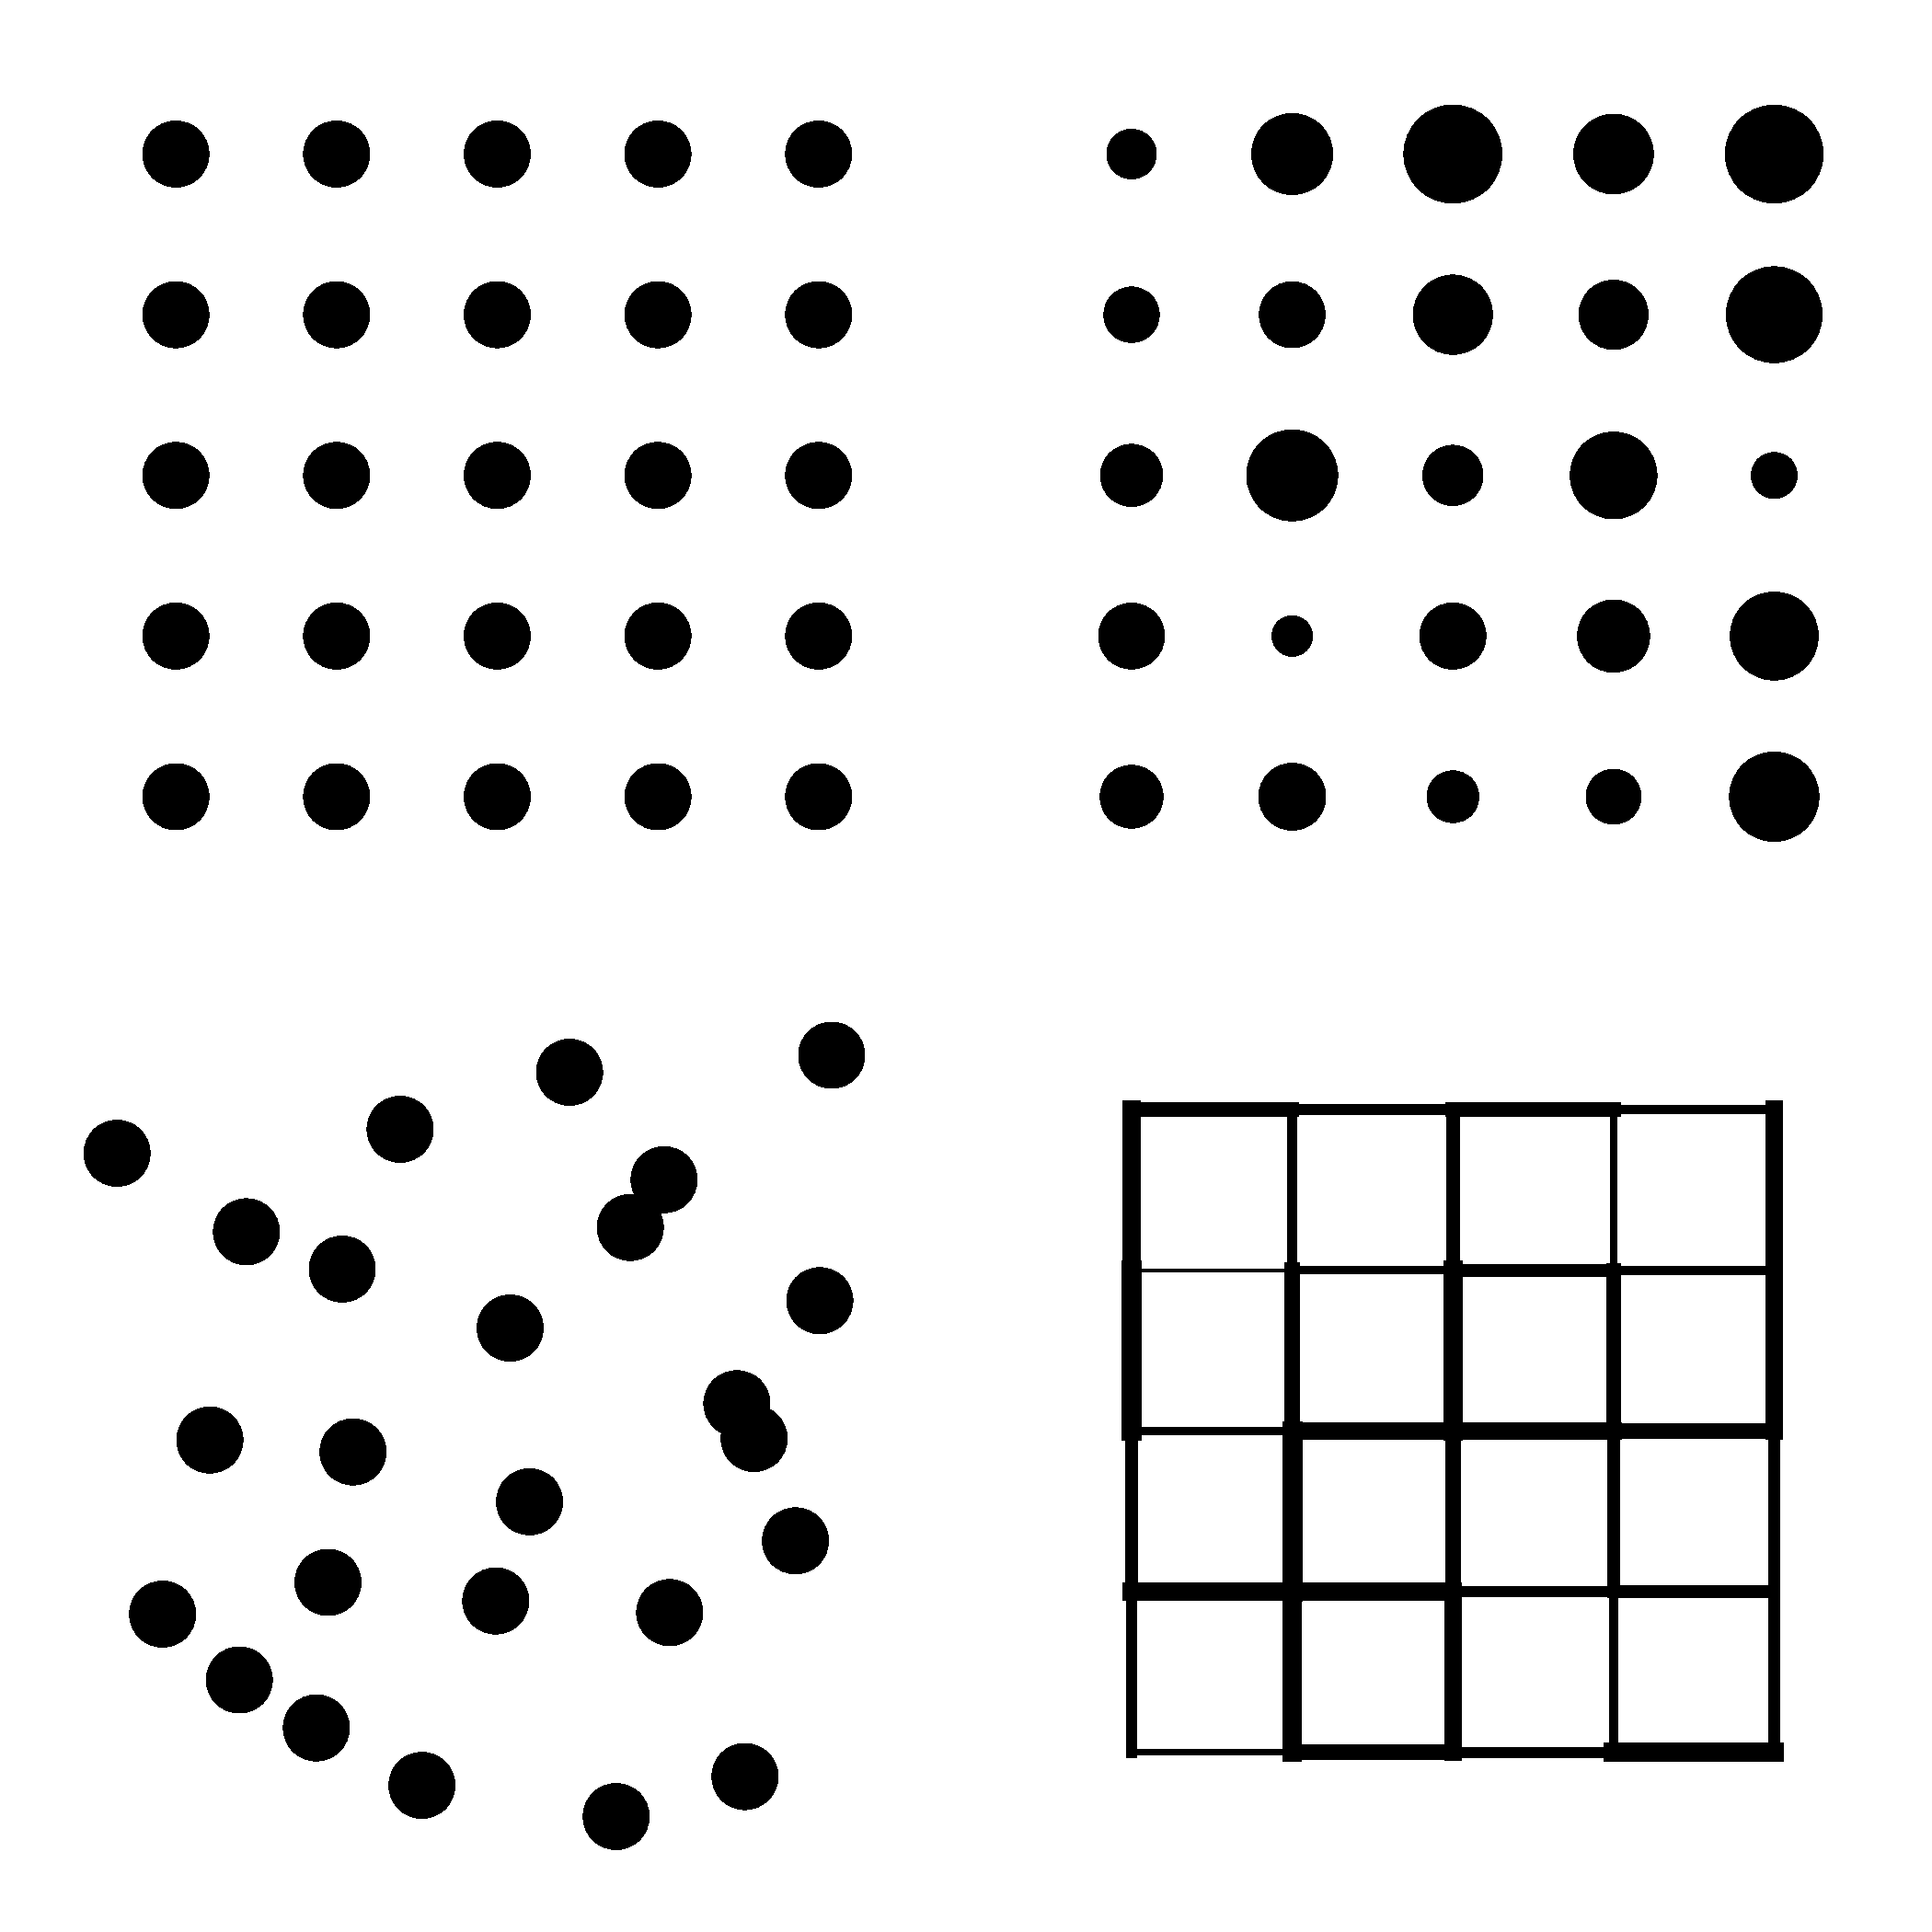
\includegraphics[width=0.7\textwidth]{disorder_scheme.pdf}}
\caption{Schematics shown from left to right and top to bottom depict the following systems: an ideal crystal, a compositionally disordered system, structurally disordered system and a system with disorder in kinetic energy.  }
\label{fig:disorder} 
\end{figure}
\end{minipage}
\subsection{Models of disorder }
% NOTE:MAKE A DISTINCTION BETWEEN TYPES OF DISORDER - amplitude and concentration of defects
In ideally ordered crystalline systems of non-interacting particles, characterization of their properties is made comparatively simple by their translational symmetry. One-electron wave functions are of the Bloch type and thus the electrons are itinerant and can move in an unrestricted manner throughout such systems. In most actual systems, however, at least some degree of symmetry-breaking disorder is present, which can change the system's properties considerably. For systems with a low concentration of defects, on can still use the concepts of translationally invariant systems as a starting point in providing a description of the distorted systems. On the other hand, when the concentration of the distortions is large, one needs to abandon the translational symmetry altogether and new methods need to be developed. \\\\
\noindent As shown in Fig. \ref{fig:disorder}, various models of disorder can be constructed by somehow distorting the ideal crystal structure. By relaxing the lattice structure, models of \emph{structurally} disordered systems, such as amorphous semiconductors, can be obtained. In the continuous space representation, the one-particle Hamiltonian of such a system is given by
\begin{equation}\label{eq:amorphous_hamiltonian}
H=\frac{\hat{p}^2}{2m} + \sum\limits_{j=1}^N V_j(\mathbf{r}-\mathbf{R}_j),  
\end{equation}
where $\hat{p}$ is the momentum operator, $m$ particle's effective mass and $V_j$ the potential energy of an atom at the site $\mathbf{R}_j$. Disorder is introduced by taking both the potential energies and the site positions $\mathbf{R_j}$ at random and assuming some normalized probability density distribution function for the atomic potentials. In the case when a simple uniform probability distribution function is used, the model is used extensively in the theory of \emph{weak localization}, which will be addressed later in this seminar. \\\\
\noindent A different model is used in the studies of \emph{compositionaly} disordered solids, which are also subject of this seminar's numerical calculations. Such systems are most often described by the following tight-binding Hamiltonian on a discrete lattice:
% MAKE A DISTINCTION WITH THE PREVIOUS EQUATION
\begin{equation}\label{eq:compositional}
H=\sum\limits_{j\nu}\varepsilon_{j\nu} c^\dagger_{j\nu}c_{j\nu} + \sum\limits_{j\nu,k\mu} V_{j\nu, k\mu}c^\dagger_{j\nu}c_{k\mu}.
\end{equation}
% Here, $c^\dagger_{j,\nu}, c_{j,\nu}$ are fermionic creation and annihilation operators for a lattice site $j$ and state $\nu$. Labelled with $\varepsilon_{j\nu}$ in the diagonal part are the energies associated with states occupying particular lattice sites. The non-diagonal matrix elements $V_{j\nu, k\mu}$ correspond to quantum tunnelling transitions between states at different sites. Disorder is introduced by taking the site energies or hopping matrix elements (or both) at random and assumming some probability distribution for them. In our case, we consider the case of purely diagonal disorder with nearest-neighbour hoppint at a constant rate $V$, and with only one contributing one-electron orbital, $\nu=1$. According to the Anderson model, site energies $\varepsilon_j$ are drawn uniformly from the interval $[-W,W]$ according to the probability density function $p(\varepsilon_j)=\frac{1}{2W}\Theta(W-|\varepsilon_j|)$. Our model Hamiltonian thus has the form 
% \begin{equation}\label{eq:anderson}
% H=\sum\limits_j \varepsilon_j c^\dagger_jc_j + V\sum\limits_{\text{n.n.}} c^\dagger_{i}c_j + \text{h.c.}
% % NOTE: WRITE CORRECTLY FOR NEAREST NEIGHBOUR INTERACTIONS IN ALL DIMENSIONS!!!
% \end{equation}
\begin{minipage}[t]{0.5\textwidth} 
Here, $c^\dagger_{j,\nu}, c_{j,\nu}$ are fermionic creation and annihilation operators for a lattice site $j$ and state $\nu$. Labelled with $\varepsilon_{j\nu}$ in the diagonal part are the energies associated with states occupying particular lattice sites. The non-diagonal matrix elements $V_{j\nu, k\mu}$ correspond to quantum tunnelling transitions between states at different sites. Disorder is introduced by taking the site energies or hopping matrix elements (or both) at random and assumming some probability distribution for them. In contrast to the model given by Eg. \eqref{eq:amorphous_hamiltonian}, however, there is no structural disorder - lattice sites reside on well-defined positions in an ordered crystal lattice. \\\\
\noindent The \textbf{Anderson model} is obtained from the one given in Eq. \eqref{eq:compositional} by assuming purely diagonal disorder with 
nearest-neighbour hopping at a constant rate $V$ and only one contributing 
% In our case, we will be dealing with the \textbf{Anderson model} consider the case of purely diagonal disorder with nearest-neighbour hopping at a constant rate $V$, and with only one contributing one-electron orbital, $\nu=1$. In the Anderson model, site
\end{minipage}\hfill
\begin{minipage}[t]{0.45\textwidth}
\begin{figure}[H]
\centering{
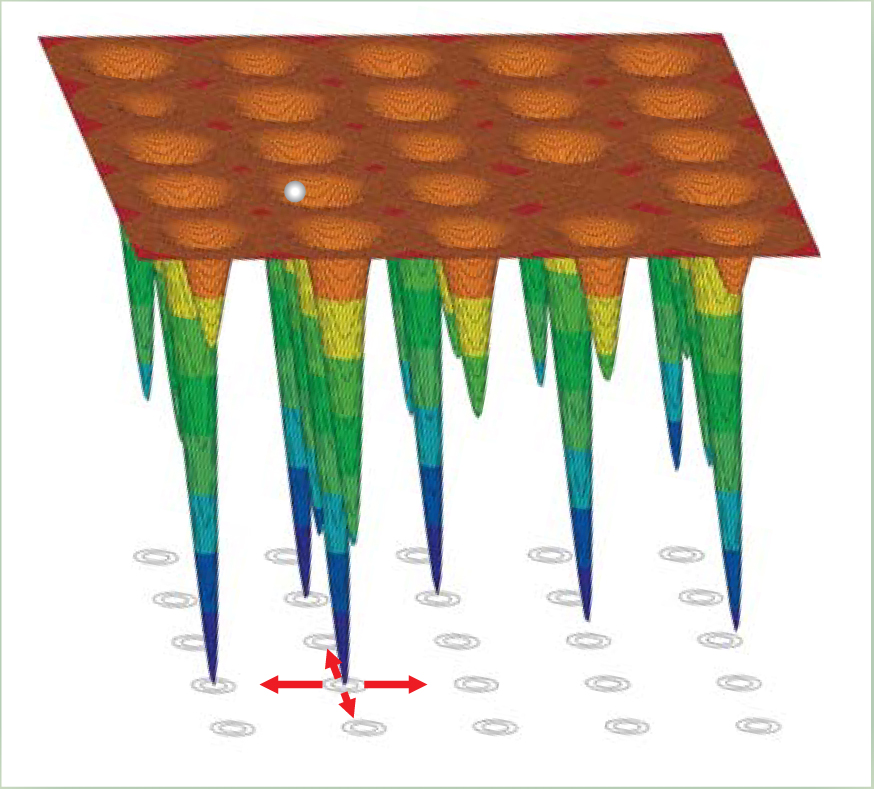
\includegraphics[width=0.65\textwidth]{hopping_picture_50years.jpg}}
\caption{A cartoon representing the physics of the Anderson model given by Eq. \eqref{eq:anderson}. A particle on an ordered lattice can hop to the nearest sites which have randomly varying site energies. Image was taken from \cite{50yearsof}.}
\label{fig:disorder} 
\end{figure}
\end{minipage}
\noindent  one-electron orbital, $\nu=1$. Site
energies  $\varepsilon_j$ are drawn uniformly from the interval $[-W,W]$ according to the probability density function 
\begin{equation}\label{eq:probability}
p(\varepsilon_j)=\frac{1}{2W}\Theta(W-|\varepsilon_j|),
\end{equation}
where $W$ is the disorder-strength parameter. Our model Hamiltonian thus has the form 
\begin{equation}\label{eq:anderson}
H=\sum\limits_j \varepsilon_j c^\dagger_jc_j + V\sum\limits_{\text{n.n.}} c^\dagger_{i}c_j + \text{h.c.}
\end{equation}
Unless explicitly specified, Hamiltonian given by Eq. \eqref{eq:anderson} is the one we will be reffering to in the subsequent sections of the seminar. 
\subsection{Conductivity before and after the localization theory }
%to do: first: interference effects, quantum coherent back-scattering (weak localization), then strong localization; always reffer to the model structure and the tight-binding picture (see Mott, Davis) as this should be known from Condensed matter course; then proceed onto the introduction of the mobilty edge concept which is related to the band structure
The localization of quantum particles by a static random potential is an intriguing phenomenon of statistical physics. Prior to the advent of the Anderson theory of localization, the electronic conductance was described in terms of the quantum-mechanical revision of the classical Drude model. The latter assummes the electronic conductivity should be directly proportional to the mean-free path $l$, the average distance a particle travels before colliding with an impurity. Quantum-mechanically, wave packets propagating through a disordered medium will be scattered by the random potential on average after traveling a distance $l$. This would cause them to lose their well-defined momentum, however, the wave functions should remain extended throughout the system despite the scattering. Such propagation is diffusive on larger length scales and while increasing disorder should therefore lower the conductivity by lowering the mean-free path, the conductivity should remain finite for any finite disorder. This traditional description of conduction in disordered systems turns out to be incorrect as shown by Anderson in 1958. In case of a sufficiently strong disorder, particles in a system may become localized with their wave function's envelope decaying exponentially from some point $\mathbf{r}_0$ in space as $|\psi(\mathbf{r})| \sim \exp\left(|\mathbf{r} - \mathbf{r}_0 |/\xi \right)$, where $\xi$ is the \emph{localization length}. In that case, diffusive particle propagation is not only reduced, but can come to a complete halt - the particle becomes trapped and the conductivity vanishes. In order to see how this rather striking result comes about, one needs to consider multiple interference of wave components scattered by randomly placed scattering centers - localization is foremost an interference phenomenon.
\subsubsection{Enhanced back-scattering }
The importance of quantum interference in the onset of Anderson localization can be most clearly recognized in the limit of weak disorder and consequent weak scattering. Starting with elementary wave mechanics, let us suppose an electron is propagating in a disordered medium from point $\mathbf{r}_0$ to 
\begin{minipage}[t]{0.58\textwidth} 
point $\mathbf{r}_1$. To obtain the total probability of electron's arrival at $\mathbf{r}_1$, one needs to sum the complex-valued probability amplitudes of all paths between the two points and square the complex-valued end result. The final probability consists of a sum of squares of individual amplitudes - the classical, inchorent contribution - together with many cross-product, interference terms. In most cases, one can safely assume that the phases of interference terms are distributed randomly in a disordered medium and hence their sum vanishes on average. Such an omission of interference terms restores thetraditional description of conductivity in disordered systems and is obviously not always justified. Let us consider the probability amplitude $A_1$ for a particle starting at $\mathbf{r}_0$ to move along some path $C_1$ and returning back to the starting point and the probability amplitude $A_2$ to move along some other path
\end{minipage}\hfill
\begin{minipage}[t]{0.39\textwidth}
\begin{figure}[H]
\centering{
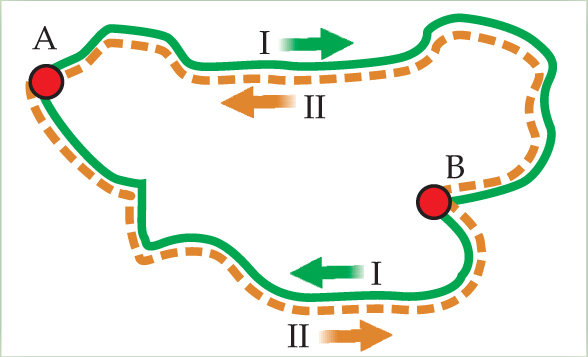
\includegraphics[width=0.9\textwidth]{interference.jpg}}
\caption{A schematic of a wave packet propagating from point A through point B back to A along path I and along its time-reverse II. Image was taken from \cite{50yearsof}.}
\label{fig:paths} 
\end{figure}
\end{minipage}
 $C_2$, as shown in Fig. \ref{fig:paths}. The return probability for the two possible returning paths will be 
\begin{equation}
w=|A_1 + A_2|^2=w_\mathrm{cl} + w_\mathrm{int},
\end{equation}
with $w_\mathrm{cl}=|A_1|^2 + |A_2|^2$ and $w_\mathrm{int}=2\Re\left(A_1^*A_2\right)$. For different returning paths $C_1$ and $C_2$, the interference terms of many such combinations average out, as discussed above. However, if $A_2=A_r$ is the amplitude for a time-reversed path $C_1$ and the system is time-reversal invariant, $A_1=A_r$, then the proper consideration of interference terms yields a twice larger return probability than in the classical case:
\begin{equation}
w=4|A_1|^2=2w_\mathrm{cl}.
\end{equation}
In a scattering event, an outcome of an electron scattering back to its initial point is thus slighlty more likely than all other outcomes due to the constructive interference of a path with its time-reversed counterpart, which is often reffered to as the \emph{enhanced back-scattering}. The effect lowers the electron's transmission probability and hence also reduces conductivity. 
% \noindent The above discussion is valid if the propagation is phase-coherent, meaning that the phase is not altered in a random manner during scattering events. This is the case if the scattering is static, e.g. the scatterers have no internal degrees of freedom, such as spins or phonons. In the zero-temperature limit, this effect alone leads to exponential localization of all states in one and two dimensions for any finite disorder. 
\subsection{Existence of the mobility edge}
\begin{minipage}[t]{0.5\textwidth} 
In three dimensions, as shown by Anderson \cite{Anderson}, localization of all states only occurs if compositional disorder is sufficiently strong. For weaker values of disorder, both localized and extended states exist in the system where $E_c$, or the \emph{mobility edge}, is the critical energy determining whether a state is localized or not. To provide at least a qualitative justification for the existence of a mobility edge, let us now examine the tight-binding Hamiltonian given by Eq. \eqref{eq:anderson} in more detail. In lattice systems, a tight-binding Hamiltonian is an ideal array of equal potential wells, as shown in \textbf{a)} in Fig. \ref{fig:band_structure}. Energies of such a system are obtained by diagonalizing the Hamiltonian at $W=0$ using the Fourier transform. The dispersion relation for a system with a simple cubic unit cell of length $a$ is given by
\begin{equation}\label{eq:dispersion_crystal}
E_\textbf{k}=-2V\left(\cos(k_x a) +\cos(k_y a) +\cos(k_z a)\right).
\end{equation}
\end{minipage}\hfill
\begin{minipage}[t]{0.45\textwidth} 
\begin{figure}[H]
\centering{
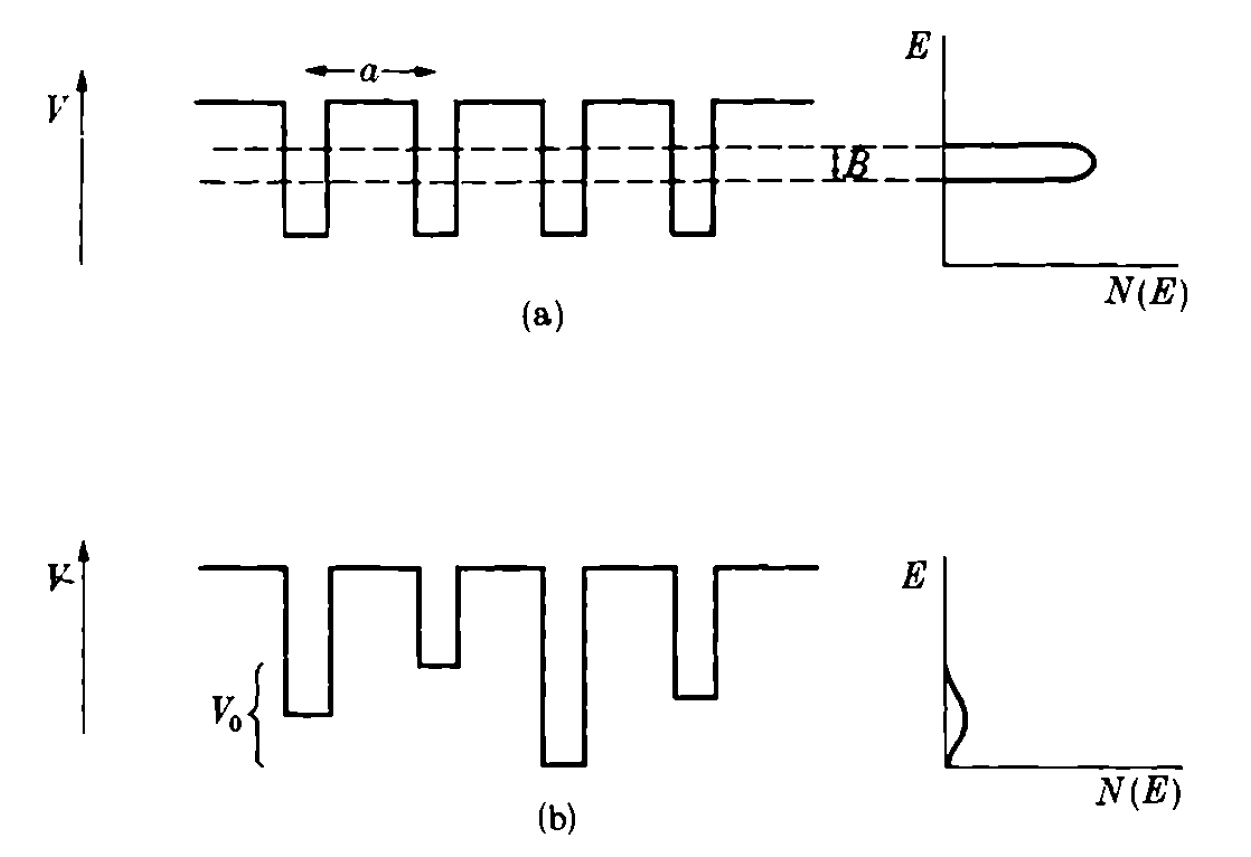
\includegraphics[width=1\textwidth]{bands.png}}
\caption{a) Potential wells in the tight-binding approximation in an ideal crystalline lattice. b) Potential wells for the Anderson lattice with randomly varying potential strengths. Image was taken from \cite{Mott}.  }
\label{fig:band_structure} 
\end{figure}
\end{minipage}\\\\
In general, the energies form a narrow band of width $2zV$, where $z$ is the coordination number. Wave functions of such a system are Bloch waves  
\begin{equation}\label{eq:Bloch}
\psi_k(\mathbf{r})= \sum_j\exp(\mathrm{i}\mathbf{k}\cdot\mathbf{R_j})\phi(\mathbf{r}-\mathbf{R}_j),
\end{equation}
where $\phi$ are the spherically symmetric one-electron wave functions. As shown in \textbf{b)} in Fig. \ref{fig:band_structure}, compositional disorder is introduced to the system by randomly changing the depths of each potential well by some value $\varepsilon_j$ drawn from the interval $[-W,W]$ according to the distribution given by Eq. \eqref{eq:probability}. As shown in Fig. \ref{fig:accidental_wells}, random variations of the site potential form accidental potential wells, in which particles may become localized. The amplitude of the variations depends on the value of the disorder parameter $W$ - for small $W$ in the case of weak disorder, only small potential fluctuations are introduced, whereas for large $W$ the site energies at neighbouring sites can differ significantly and thus deep potential wells may be formed. It is instructive to first consider the limit of very strong disorder, in which the onset of localization can be grasped rather intuitively.\\\\
% \begin{minipage}[t]{0.58\textwidth} 
% In three dimensions, as shown by Anderson \cite{Anderson}, localization of all states only occurs if compositional disorder is sufficiently strong. For weaker values of disorder, both localized and extended states exist in the system where $E_c$, or the \emph{mobility edge}, is the critical energy determining whether a state is localized or not. To provide at least a qualitative justification for the existence of a mobility edge, let us now examine the model tight-binding Hamiltonian given by Eq. \eqref{eq:anderson} in more detail. In an ordered system, a tight-binding Hamiltonian is an ideal array of equal potential wells, as shown in \textbf{a)} in Fig. \ref{fig:band_structure}. Energies of such a system form a narrow band of width $2zV$, where $z$ is the coordination number, and its wavefunctions are the Bloch waves 
% \begin{equation}\label{eq:Bloch}
% \psi_k(\mathbf{r})= \sum_j\exp(\mathrm{i}\mathbf{k}\cdot\mathbf{R_j})\phi(\mathbf{r}-\mathbf{R}_j),
% \end{equation}
%  where $\phi$ are the spherically symmetric one-electron wave functions. As shown in \textbf{b)} in Fig. \ref{fig:band_structure}, compositional disorder is introduced to the system by randomly changing the depths of each potential well by some value $\varepsilon_j$ drawn from the interval $[-W,W]$ according distribution given by Eq. \eqref{eq:probability}. As shown in Fig. \ref{fig:accidental_wells}, random variations of the site potential form accidental potential wells, in which particles may become localized. The amplitude of the variations depends on the value of the disorder parameter $W$ - for small $W$ in the case of weak disorder, only small potential fluctuations are introduced, whereas for large $W$ the site energies at neighbouring sites can differ significantly and thus deep potential 
% % Following Anderson's argument, we take the tight-binding Hamiltonian given by Eq. \eqref{eq:anderson} and recall that the tight-binding Hamiltonian of an ordered system is a crystalline array of equal potential wells, which produces a narrow band of energy levels, as shown in \textbf{a)} in Fig. \ref{fig:band_structure}. Our model Hamiltonian is obtained by randomly changing the depth of each potential well by a value $\varepsilon_j$ drawn from the distribution \eqref{eq:probability}.	
% \end{minipage}\hfill
% \begin{minipage}[t]{0.38\textwidth} 
% \begin{figure}[H]
% \centering{
% 
\includegraphics[width=.6\textwidth]{dummy.pdf}}
% \caption{a) Potential wells in the tight-binding approximation in an ideal crystalline lattice. b) Potential wells for the Anderson lattice with randomly varying potential strengths.  }
% \label{fig:band_structure} 
% \end{figure}
% \begin{figure}[H]
% \centering{
% 
\includegraphics[width=.61\textwidth]{dummy.pdf}}
% \caption{Qualitative picture of the Anderson model density of states. States in the band tails are localized while those in the middle are localized. $E_c$ and $E_c'$ are the mobility edges. }
% \label{fig:band_edges} 
% \end{figure}
% \end{minipage}
\noindent 
\begin{minipage}[t]{0.58\textwidth}
\noindent In the limit of very strong disorder, where disorder strength is determined relative to the hopping rate $V$, we can assume that the potential term in Eq. \eqref{eq:anderson} strongly prevails over the hopping term and thus localization of states is preffered. In that case, a zeroth order description of the Hamiltonian's eigenfunction would be a bound state or a localized orbital bound by some deep fluctuation in the random potential. The one-electron orbitals do not hybridize into extended states since orbitals that are nearby in space and thus
% The nondiagonal Hamiltonian terms, which generally contribute towards hybridization of one-electronic orbitals into extended states and towards the formation of energy bands, can be treated as a weak perturbation and have a practically negligible effect in this limit. For hybdridization to occur, two key conditions must be met. 
have a considerable overlap usually differ significantly in energy. States with similar energies, on the other hand, are usually spatially distant and hence overlap negligibly. Failing to hybdridize, the states remain exponentially localized in this regime. \\\\
\noindent For intermediate disorder, both localized and extended states exist in the system with the former near the band  
\end{minipage}\hfill
\begin{minipage}[t]{0.4\textwidth}
\begin{figure}[H]
\centering{
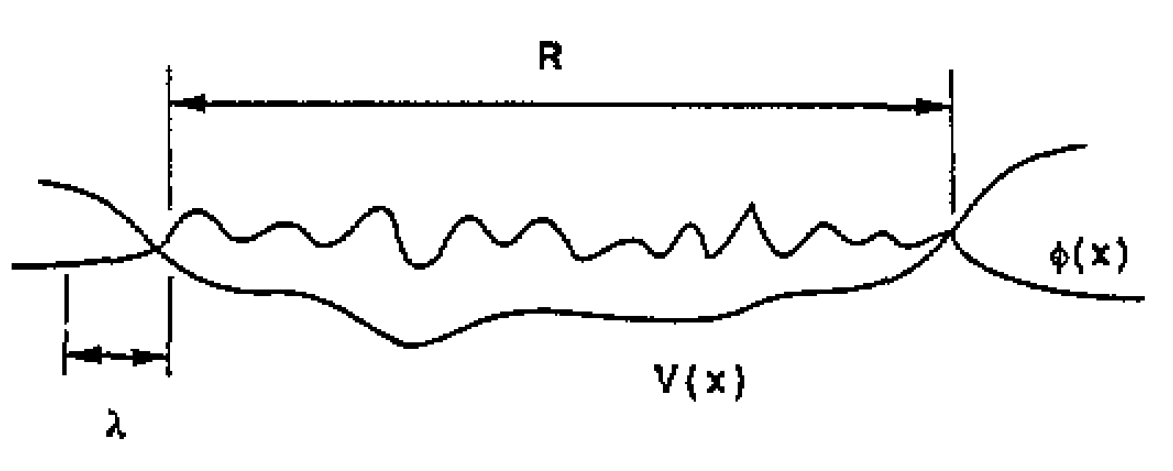
\includegraphics[width=1\textwidth]{accidental_wells.png}}
\caption{In a compositionally disordered medium, the site potential energy varies randomly from site to site. Accidental potential wells can be formed outside of which wave functions are not of oscillating, but of exponentially decaying character instead. Image was taken from \cite{Kramer}.}
\label{fig:accidental_wells} 
\end{figure}
\end{minipage}
\\\\
\begin{minipage}[t]{0.48\textwidth}
\noindent extrema and the latter near the band center. The two types of states cannot coexist at the same energies and are separated by the two critical energies $E_c$ and $E'_c$, or the mobility edges, as shown in a schematic of a typical density of states (DOS) in a disordered system in Fig. \ref{fig:DOS}. For small values of disorder parameter, it is reasonable to expect that the rather shallow accidental potential wells formed by the random potential can only localize the low-energy electron states in the left-hand tail of the DOS distribution, while a weak random perturbation is unlikely to change the extended character of the states near the band center. A localized state with the same energy as some extended state could hybridize with the latter due to their spatial overlap and matching of energies, which would in turn produce another extended state. Localized states can thus only be observed if their energies are separated from the energies of the extended states. The reason for the existence of two mobility edges, which are symmetric with respect to the band center, lies in the \emph{particle-hole} symmetry of the Hamiltonian given by Eq. \eqref{eq:anderson}.
\end{minipage}\hfill
\begin{minipage}[t]{0.5\textwidth}
\begin{figure}[H]
\centering{
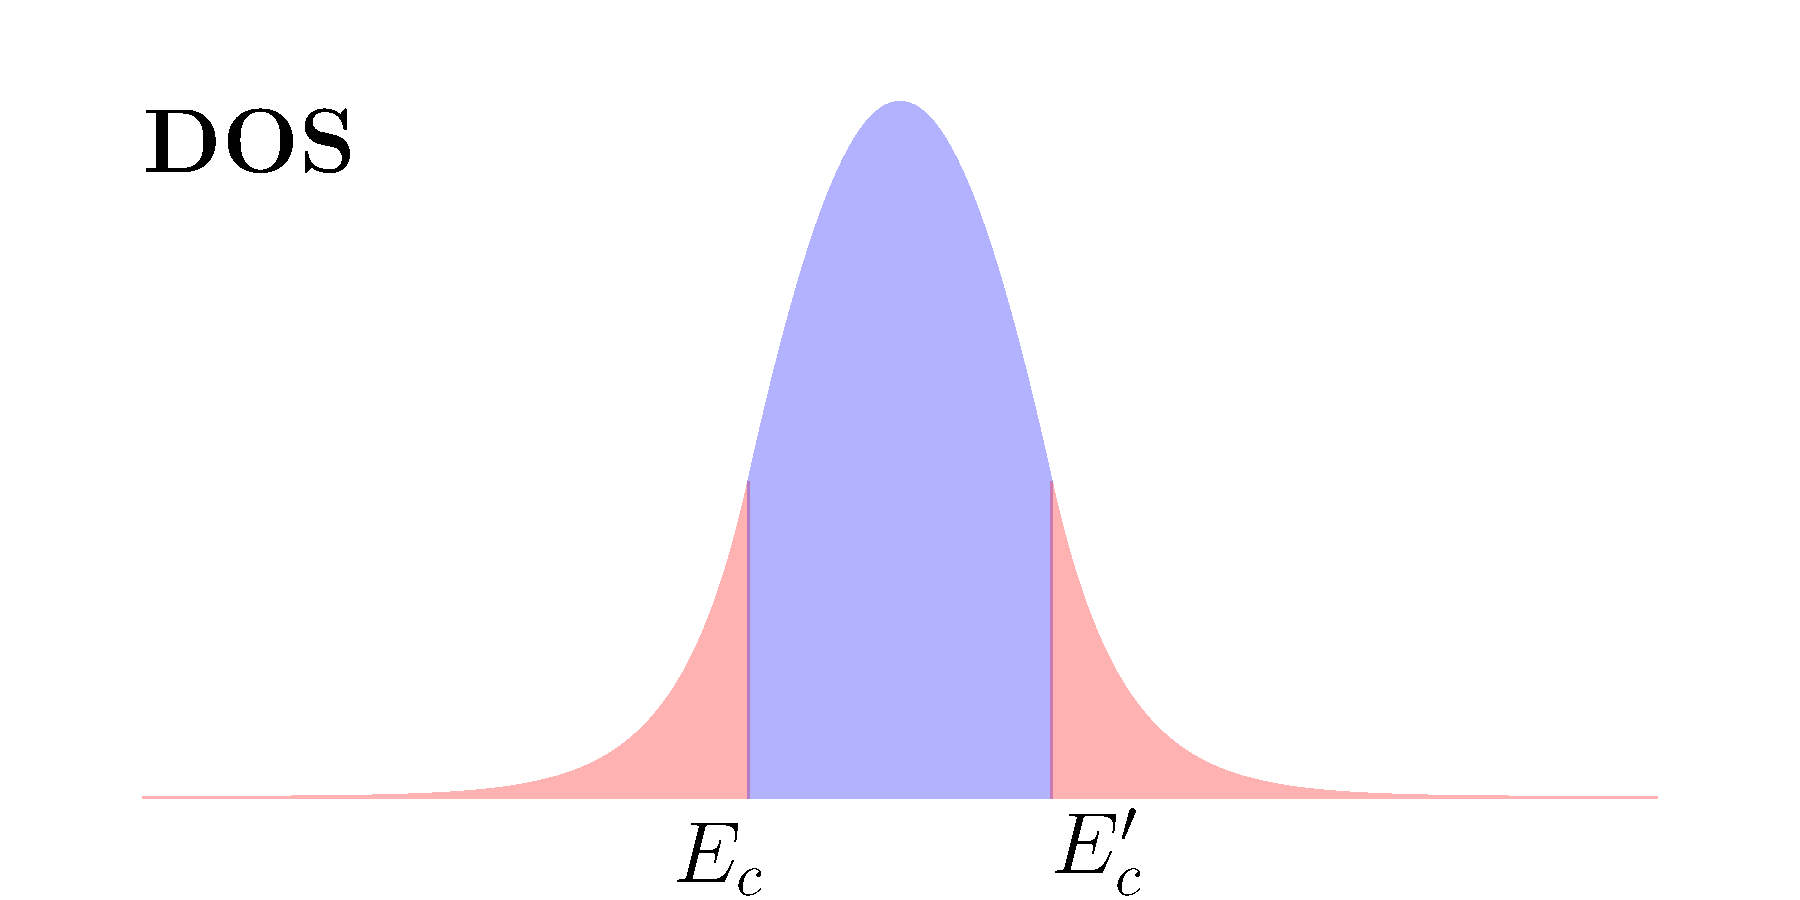
\includegraphics[width=1\textwidth]{mobility_edge_DOS.pdf}}
\caption{A schematic of a typical DOS distribution with respect to energy in the regime of intermediate disorder. A famous argument due to Lifshitz is outlined in \cite[~Section 4.2]{Kramer}, stating that the tails of the DOS distribution are falling off exponentially in a disordered system. Two mobility edges $E_c$ and $E'_c$ separate the localized and extended states. For weak disorder, only states in the exponentially decaying Lifshitz tails (coloured red) are localized while states in the center of the band (coloured blue) remain extended. Increasing $W$ eventually leads to vanishing of the blue region causing full localization to occur.  }
\label{fig:DOS} 
\end{figure}
\end{minipage}
The Anderson Hamiltonian preserves its form if electron creation and annihilation operators are replaced by their hole counterparts, according to the rule $c_j\rightarrow d_j^\dagger$, $c_j^\dagger \rightarrow d_j$, which simply establishes that a removal of an electron from the lattice corresponds to a creation of a hole. Due to the particle-hole symmetry, the physics of the electrons near the band minimum is equivalent to the physics of holes near the band maximum. This in turn means that if a critical energy $E_c$ exists describing the localization of electrons, an equivalent quantity $E'_c$ must exist describing the localization of holes. 
 % \noindent Based on rather heuristic grounds, arguments for the existence of localized states in a disordered system have been provided above. Now we are about to establish that in the intermediate regime of disorder, both extended and localized states exist in the system, however, they cannot coexist at the same energy. We start off by considering the qualitative picture of the Anderson model density of states shown in Fig. \ref{fig:band_edges}. In contrast to the density of states of an ideally ordered system, in which the density of states has singularities at the band edges (see Fig. \eqref{fig:band_structure}), we observe no singularities here. Instead, the band edges are smoothly falling off. A famous argument due to Lifshitz is presented in \cite[~Section 4.2]{Kramer}, establishing that the fall-off is exponential. We would now want to argue that for small values of the disorder parameter $W$, only the states in the exponential band tails are likely to become localized. To that end, we again proceed by taking the case without disorder as a starting point and then consider what happens with the eigenfunctions and the eigenenergies of the Hamiltonian once the disorder is introduced. We recall that in the tight-binding approximation, the dispersion relation for an electron in a simple cubic lattice without disorder is given by
 % \begin{equation}\label{eq:dispersion_crystal}
 % E_\textbf{k}=-2V\left(\cos(k_x a) +\cos(k_y a) +\cos(k_z a)\right),
 % \end{equation}
 % where $a$ is the unit cell length and $\textbf{k}=\left(k_x,k_y,k_z\right)$ is the momentum vector assuming discrete values within the first Brillouin zone. It is immediately evident that the minimum of the dispersion relation \eqref{eq:dispersion_crystal} is at the center of the first Brillouin zone. The lowest energy for a nonzero value of $k=|\mathbf{k}|$ is determined by the lowest allowed nonzero $k$, which equals $k=\pi/L$. Here, $L$ is the crystal's length provided that the crystal is of cubic shape. We note that the simple cubic unit cell was considered mainly for the sake of simplicity of our further considerations. MISSING PART HERE; ADD HOW THIS LEADS TO LOCALIZATION!!! -I would like to point out that in the limit of weak disorder, it is unlikely that a state that was previously (before the disorder) in the band's edge should change much due to the disorder. However, as these are the low energy states, the potential fluctuations introduced above are more likely to localize them in the sense of making their k-values imaginary in some region thus causing their exponential decay. This is unlikely to happen for the high-energy states in the middle of the band, hence those states would remain extended. Once the two mobility edges merge into one, full localization occurs. JUST DON'T KNOW HOW TO PHRASE THIS CORRECTLY YET. WILL MOVE ON TO OTHER SECTIONS WHICH ARE EASIER TO FINISH.
 \subsection{The scaling theory}
As shown in the previous sections, we can expect the wave functions in strongly disordered systems to become exponentially localized. Whether the particles are localized or extended when the disorder is reduced is a much more complex problem. A rigorous proof by Mott and Twose \cite{Mott_Twose} exists stating that in one dimension, all states are localized, no matter how weak the disorder. In three dimensions, all states are localized above some critical disorder strength while both localized and extended states exist for subcritical disorder strengths. In the limit of an infinitely-sized two-dimensional system, all states seem to localize for any finite disorder while the finite-size systems may display metallic properties. So far, no rigorous proof has been given for the two-dimensional case. The dependence of localization in disordered systems on their dimensionality is obviously nontrivial, which is why a complete and rigorous theoretical treatment of the localization phenomena has yet to be developed. A rather qualitative but highly instructive insight is provided by the now widely-accepted \emph{scaling theory} of localization, which was put forth in 1979 by Abrahams, Anderson, Licciardello and Ramakrishnan \cite{scaling}. Even though the theory is based on intuitive grounds, it nevertheless succeeds in giving an elementary description of the role the dimensionality plays in localization phenomena. According to the theory, the Anderson localization transition can be described in the language of critical phenomena of continuous (quantum) phase transitions. The latter occur at zero temperature and are driven by some parameter other than temperature. If disorder strength is considered as a driving parameter, this holds true in the case of Anderson localization as well. In the language of phase transitions, the scaling theory provides scaling laws for various quantities of interest among which we shall only briefly consider the conductance in this seminar. \\\\
\noindent The scaling theory of the conductance takes the conductance itself as its scaling variable. Before proceeding, we recall that in a three-dimensional ohmic conductor, the conductivity $\sigma$, an intensive property, and conductance $g$, an extensive property, are related by $g=\sigma \frac{S}{L}$. Here, $S$ is the conductor's cross-section area and $L$ its length. To describe the conductance $g(L)$ of a $d$-dimensional hypercube of the volume $L^d$, its logarithmic derivative $\beta$ is introduced:
\begin{equation}\label{eq:beta}
\beta=\frac{\mathrm{d}\log g}{\mathrm{d}\log L}.
\end{equation}
The theory assumes that $\beta$ depends only on $g$ itself, and not explicitly on energy, disorder or $L$. Its qualitative behaviour was obtained from the known asymptotic behaviour at large and small conductances
\begin{minipage}[t]{0.57\textwidth}
while an interpolation has been made in the intermediate region, assuming that $\beta$ is a continuous, monotonically increasing function. From Eq.\eqref{eq:beta} it is evident that the conductance $g$ increases with system size if $\beta>0$, which reflects metallic character. In the metallic region, the classical relation between the conductance and the conductivity holds,
\begin{equation}\label{eq:classical}
g(L)=\sigma \frac{L^{d-1}}{L}=\sigma L^{d-2}. 
\end{equation}
The relation for a three-dimensional ohmic resistor specified above is only a special case of the more general relation given by Eq. \eqref{eq:classical}, from which we obtain $\beta=d-2$ in the metallic region. Consequently, $\beta$ is positive for three-dimensional conductors, zero for two-dimensional conductors and negative in one dimension. In the opposite limit, e.g. in the localized region, $g$ decays exponentially with system size, $g \propto \exp(-L)$, and so $\beta<0$. Its precise functional dependence in this regime 
\end{minipage}\hfill
\begin{minipage}[t]{0.42\textwidth}
\begin{figure}[H]
\centering{
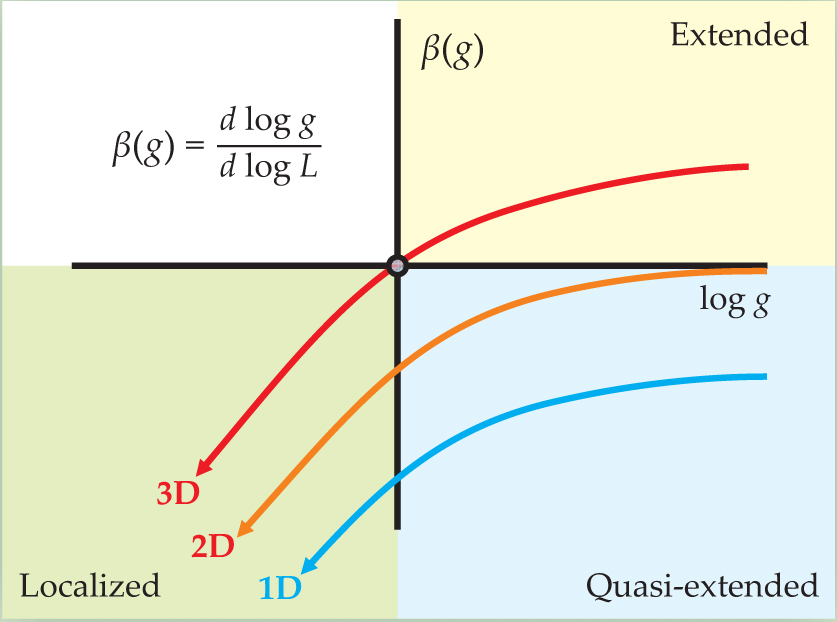
\includegraphics[width=0.8\textwidth]{beta_diagram.jpg}}
\caption{According to the scaling theory, a phase transition between a metal and an insulator can only occur in three-dimensional systems since the conductance always decreases in lower dimensional systems. Image was taken from \cite{50yearsof}.}
\label{fig:scalingtheory} 
\end{figure}
\end{minipage}
is given by
% If $\beta<0$, on the other hand, $g(L)$ decreases with $L$ and eventually terminates in the localized region, where conductance is expected to decay exponentially, $g \propto \exp(-L)$. For $\beta$ in this region, we obtain
$$
\beta=\frac{\mathrm{d}\log g}{\mathrm{d}L}\frac{\mathrm{d}L}{\mathrm{d}\log L}=\log g
$$
The transition between an insulator and a metal occurs at the critical point $\beta(g_c)=0$.  This can only happen in three dimensions where $\beta$ can assume both negative  
and positive values while conductance always decreases with system size in lower dimensional systems and so the critical point is never reached.
 \subsection{Criteria for localization}
In this section the criteria used to determine the presence of localized states in the system are presented. We focus on the two used in our numerical simulations, namely the \emph{inverse participation number} and the absence of diffusion. \\\\
\noindent Whether a state is localized or extended can be determined by considering the second moment of the probability density or the inverse participation ratio:
\begin{equation}\label{eq:inverse_part}
P^{-1}=\sum\limits_\mathbf{r} |\psi(\textbf{r})|^4, \hspace{5mm} \norm{\psi}=1.
\end{equation}
The inverse participation ratio is a measure of the portion of the space where the wavefunction differs markedly from zero and takes a value of $1$ for a wavefunction localized at a single site while its value is small for extended states. It also provides a measure for an average diameter $R$ of a state via $R=P^{1/d}$. One obtains $P=L^d$ for plane waves in which case $P$ equals the system volume. $R$ obviously diverges in the continuum limit which is considered as the representative behaviour of extended states. In our numerical simulations, Hamiltonian given by Eq. \eqref{eq:anderson} was diagonalized exactly and Eq. \eqref{eq:inverse_part} was applied to each of its eigenstates. \\\\
We have already established that localized states cannot contribute to electron transport in a disordered system. An initial localized wavefunction $\ket{\psi, 0}$, which must of course not be an eigenstate of the Hamiltonian given by Eq. \eqref{eq:anderson}, will not spread diffusively across the whole system with time if all eigenstates are localized. Instead, its average diameter $R$ will saturate at some value smaller than the system size. In our numerical simulations, an initial wavefunction with considerable probability amplitude only at a few sites in the center of the lattice was time evolved with a unitary time-evolution operator according to the scheme
\begin{equation}\label{eq:propagation}
\ket{\psi, t+\mathrm{d}t}=\exp\left(-\mathrm{i}\hat{H}\dd t\right)\ket{\psi, t}
\end{equation}
The wavefunction`s average diameter was determined by calculating the expectation value of the $\hat{R^2}$ operator, defined by
\begin{equation}\label{eq:spread}
\hat{R^2}=\sum\limits_{\mathbf{r}_j} \mathbf{r}_j^2 \hat{n}_{\mathbf{r}_j}, \hspace{10mm} R(t)=\sqrt{\bra{\psi,t} \hat{R^2}\ket{\psi,t}-\bra{\psi,0} \hat{R^2}\ket{\psi,0}},
\end{equation}
where $\hat{n}_{\mathbf{r}_j}=c^\dagger_{\mathbf{r}_j}c_{\mathbf{r}_j}$ is the particle number operator at the site $\mathbf{r}_j$. In the fully localized case, $R(t)$ eventually saturates at a finite value, while transport is ballistic in the absence of disorder with $R(t)=\sqrt{zV}t$ for a delta-function like initial wavefunction. Diffusive behaviour is expected in the intermediate regime. 
\section{Numerical simulations}
In order to test the theoretical considerations of the previous sections, numerical calculations have been performed in \url{Python}. The Anderson Hamiltonian given by Eq. \eqref{eq:anderson} with imposed open boundary conditions was considered on a finite lattice in one, two and three dimensions. For a given system size $L$ and disorder parameter $W$, the results for $P^{-1}$ and $R(t)$ were calculated. Both quantities need to be understood in terms of ensemble averages $\langle \dots \rangle$ over different realizations of random disorder since only such averaging can yield physically relevant results representative of a system with a given disorder strength $W$. Methods for calculation of $R(t)$ and $P^{-1}$ are explained in more detail below. \\\\
% Absence of diffusion in the presence of disorder was studied by time evolving an initial sharply localized wave packet according to the propagation scheme \eqref{eq:propagation} and evaluating the value of $R(t)$ given by Eq. \eqref{eq:spread} on each propagation step. Numerical package \url{sparse} for calculations involving sparse matrices from \url{Python} \url{SciPy} library has been used in our calculations since the Anderson Hamiltonian can be represented by a sparse matrix. The time-evolution operator in Eq. \eqref{eq:propagation} has been approximated by its Taylor expansion up to tenth order which proved sufficiently accurate for our calculations. The wavefunction $\ket{\psi,t}$ was renormalized on each time step to make sure that the propagation preserved its norm. 	A step-length of $\dd t=0.1$ has been used in all time-evolution simulations. \\\\
\begin{minipage}[t]{0.27\textwidth}
Absence of diffusion in the presence of disorder was studied by time evolving an initial sharply localized wave packet for a given realization of disorder given by \eqref{eq:probability}. Propagation was performed according to Eq. \eqref{eq:propagation} and the value of $R(t)$ was evaluated at each time step. Numerical package \url{sparse} for calculations involving sparse matrices from the \url{SciPy} library has been used in our calculations since the Anderson Hamiltonian can be represented by a sparse matrix. The time-evolution operator in Eq. \eqref{eq:propagation} has been 
\end{minipage}\hfill
\begin{minipage}[t]{0.72\textwidth}
\begin{figure}[H]
\centering{
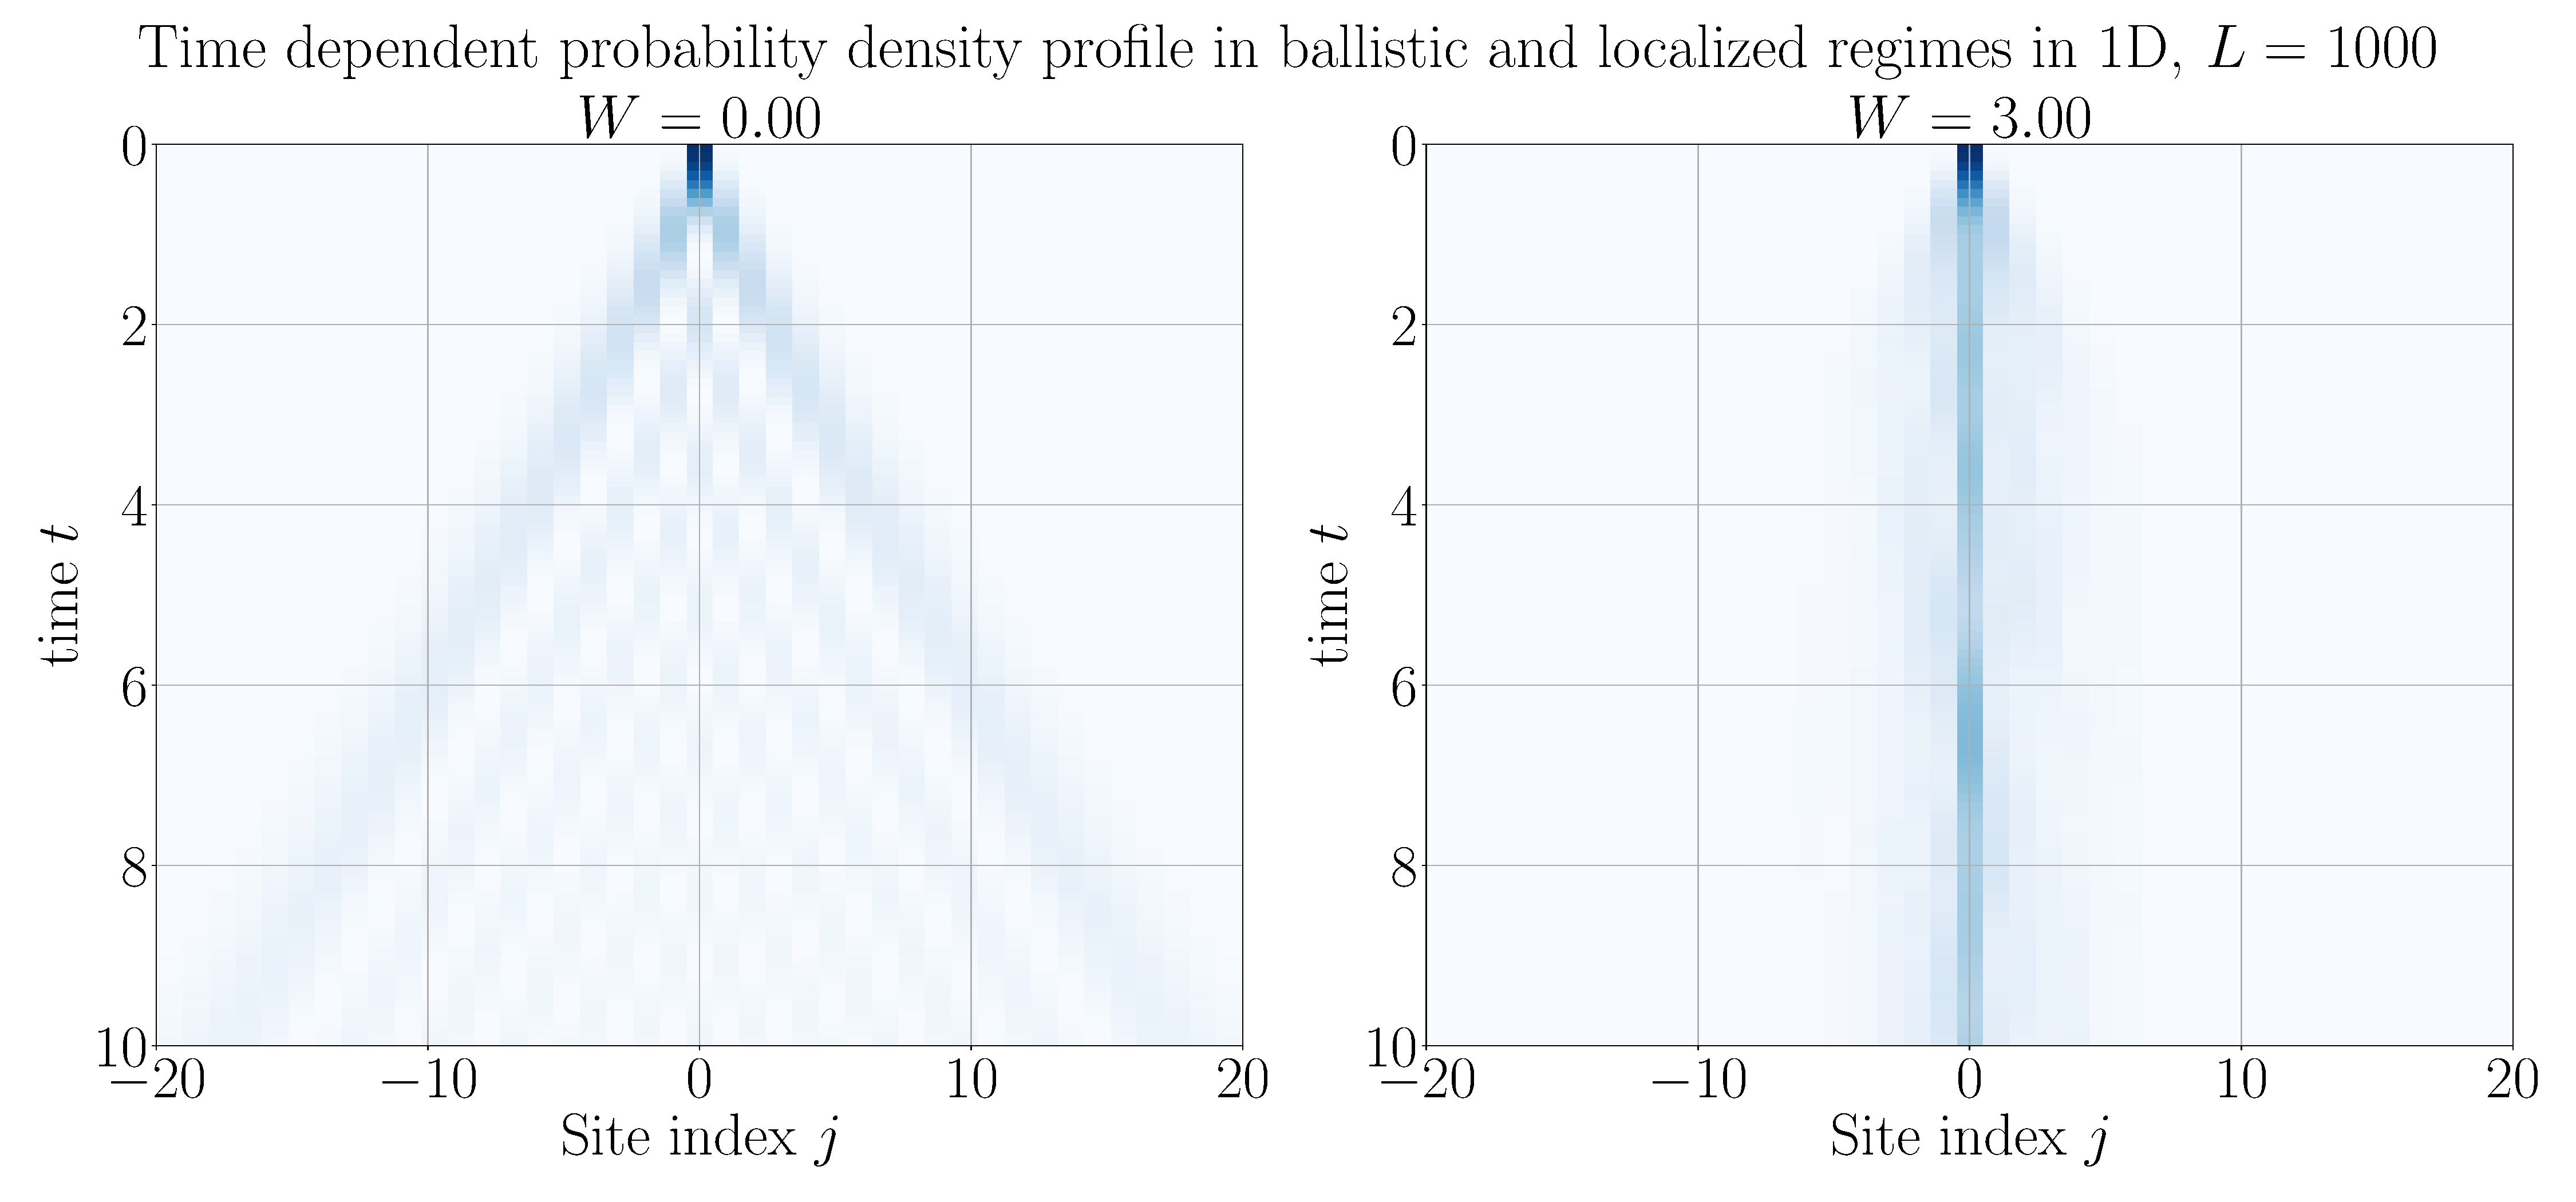
\includegraphics[width=1\textwidth]{1D_Anderson_loc_seminar_D1_shape_1000_light_cone_double.pdf}}
\caption{Time evolution of an initial delta-function like wave packet in the ballistic regime with $W=0.0$ and in the localized regime with $W=3.0$ where all eigenstates are localized due to strong disorder. While the density profile spreads out with time in the first case it remains localized around its initial site $j=0$ in the second case. }
\label{fig:light_cone} 
\end{figure}
\end{minipage}
 approximated by its Taylor expansion up to tenth order which proved sufficiently accurate for our needs, while the renormalization of $\ket{\psi,t}$ on each time step ensured the propagation preserved the wavefunction's norm. A step-length of $\dd t=0.1$ has been used in all time-evolution simulations. For a given $W$, time-dependent $R(t)$ values were obtained by averaging over 50 to 200 realizations of random disorder. Graphs in Fig. \ref{fig:light_cone} show two typical examples of time evolution in ballistic and localized regimes. \\\\
Finite-size effects in finite systems present a formidable challenge in numerically showing that localization occurs for any finite disorder strength $W$ in one and two dimensions. For small values of the disorder parameter, the wave packet may reach the lattice boundaries before it had stopped spreading, as shown in graphs in Fig. \ref{fig:1D_rsq}. This might lead one to misinterpret the result as a hallmark of absence of localization, whereas localization actually occurs on a length-scale greater than the system size. As we were unable to tackle the finite-size effects by increasing the system size further and further, we resorted to studying the time-dependence of the scaling exponent $\beta(t)$ in the leading term of the $R(t)$ dependence:
\begin{equation}\label{eq:beta}
R(t)\approx At^{\beta(t)}+\dots
\end{equation}
The value of $\beta$ is identically equal to 1 at all times in the ballistic case and should monotonically decrease in time towards the value of zero for any finite disorder. In actual simulations, this only holds true for as long as the finite-size effects are absent. The results of the simulations in the one-dimensional case are shown in Fig. \ref{fig:1D_rsq}.\\\\
% \begin{figure}[H]
% \floatbox[{\capbeside\thisfloatsetup{capbesideposition={left,center},capbesidewidth=2.3cm}}]{figure}[\FBwidth]
% {\caption{Left: time dependence of $R(t)$ for different values of $W$. Finite size effects are prominent in the $W=0.0$ and $W=0.1$ case }\label{fig:1D_rsq}}
% {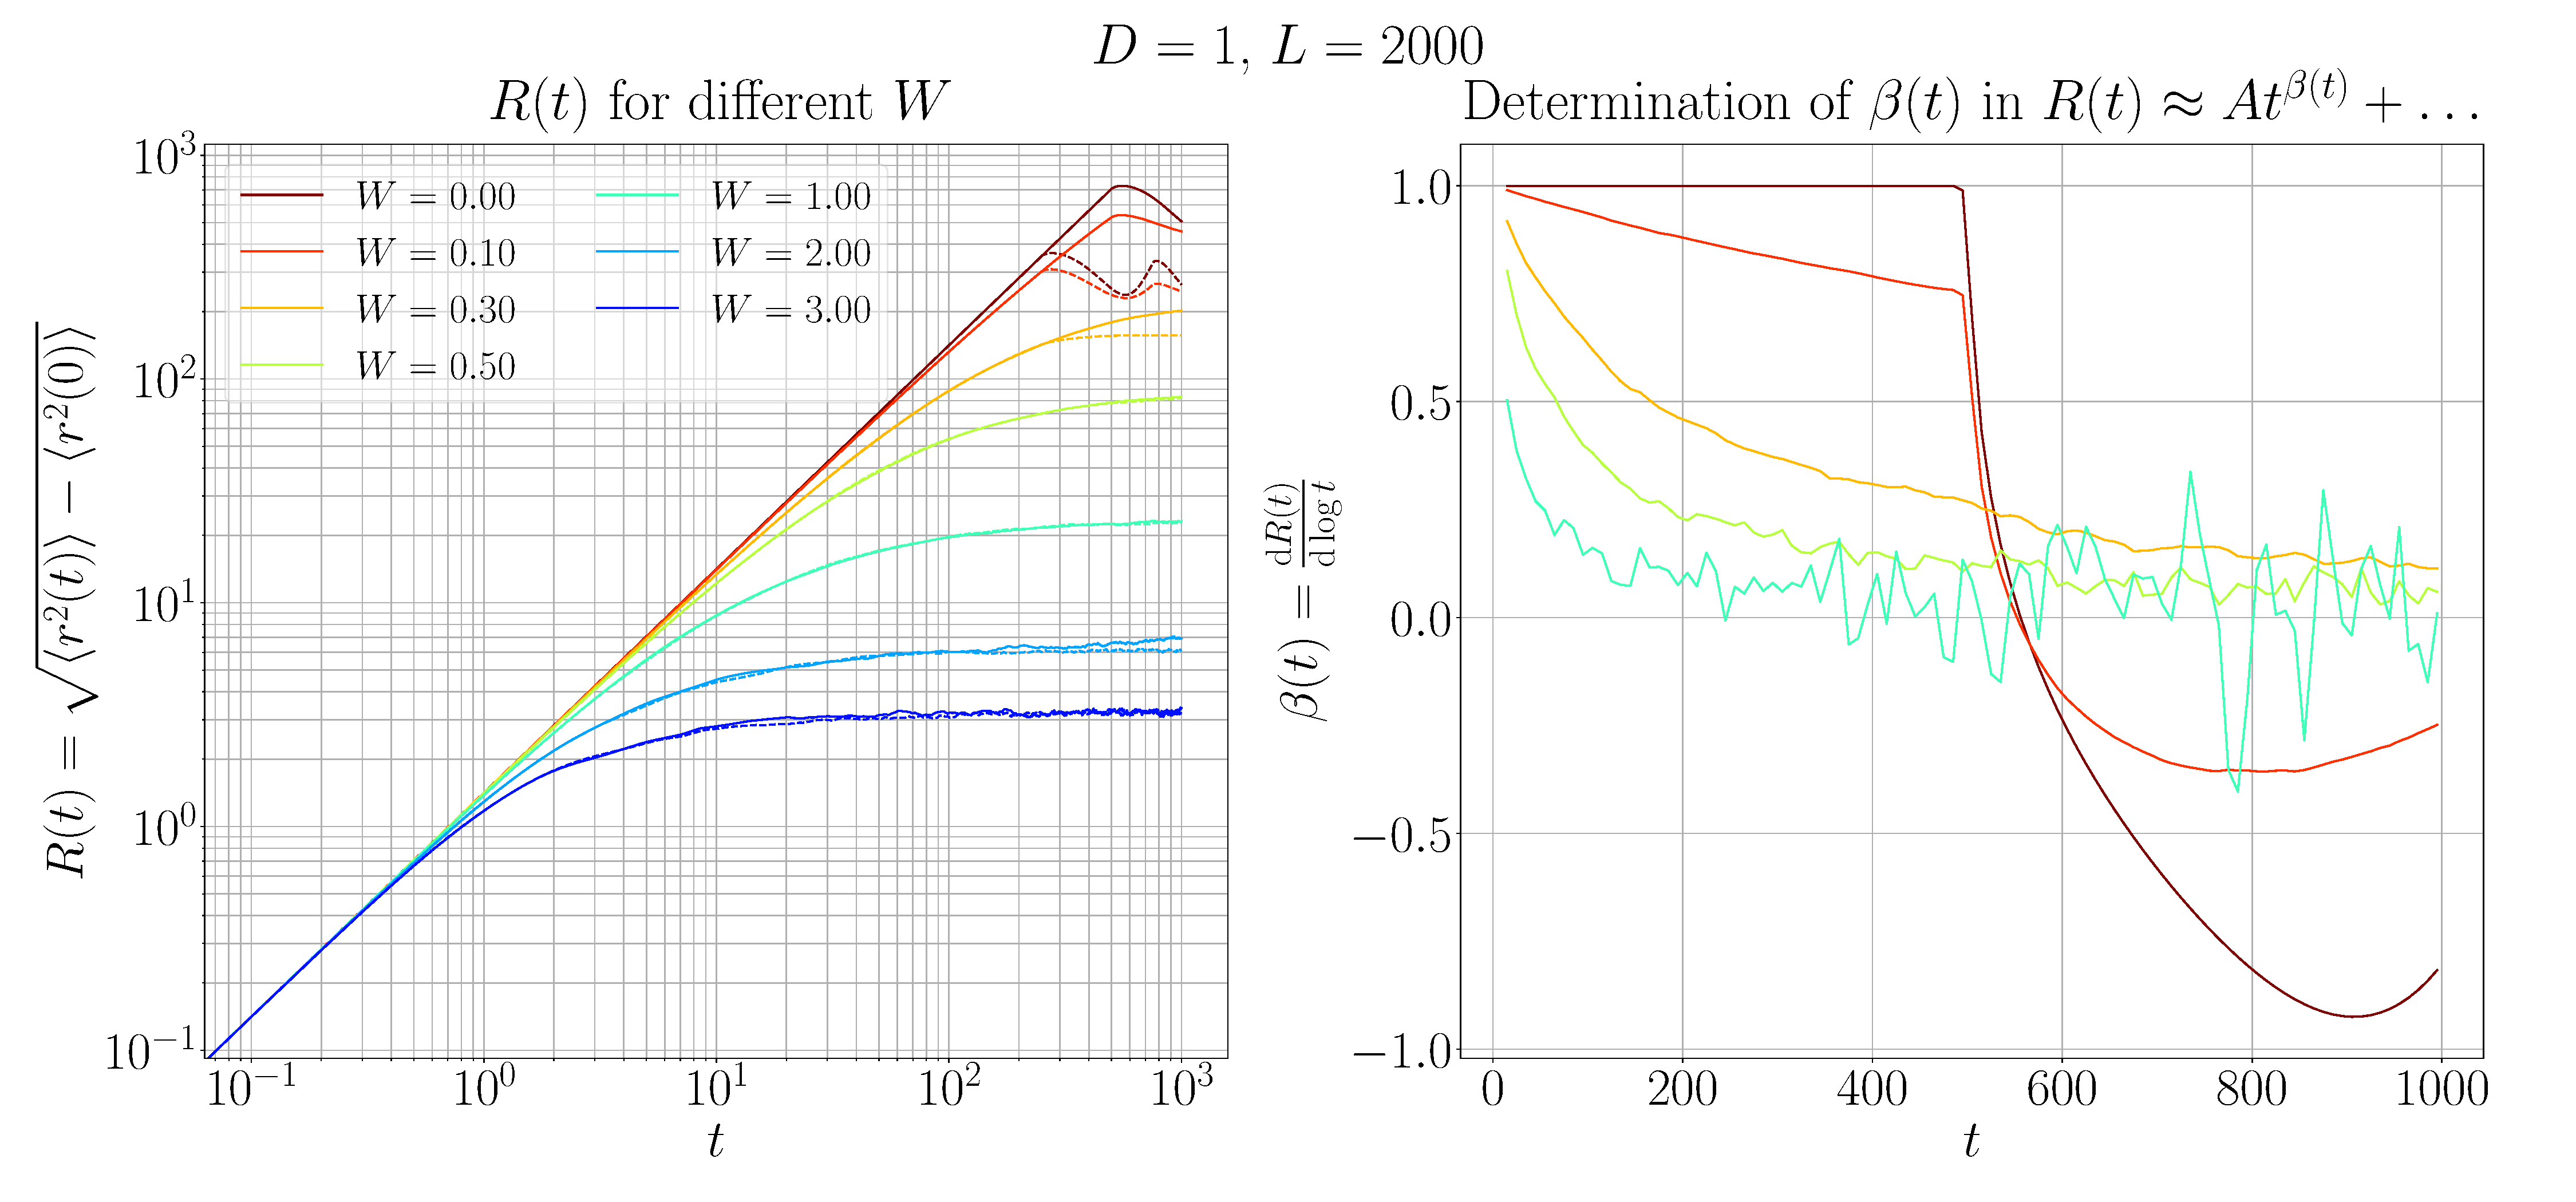
\includegraphics[width=0.85\textwidth]{1D_Anderson_localization_Seminar_scaling_analysis_D1_shape_2000_r_sq_dynamics.pdf}}
% \end{figure}
\noindent
Studies of the inverse participation ratio $P^{-1}$ have been performed by first diagonalizing the Anderson Hamiltonian for a given realization of disorder:
\begin{equation}
\hat{H}\ket{\psi_\alpha} = E_\alpha\ket{\psi_\alpha}.
\end{equation}
Here, $E_\alpha$ and $\ket{\psi_\alpha}$ denote the Hamiltonian's eigenenergies and eigenstates, respectively. Numerical diagonalization was carried out using the routine \url{eigh()} from the package \url{numPy.linalg}. Each eigenstates' inverse participation ratio $P^{-1}_{\alpha}$ was then calculated according to Eq. \eqref{eq:inverse_part}. The end results were obtained by averaging $P^{-1}_{\alpha}$ values over different realizations of disorder. Finite-size analysis was done by repeating the above procedure for different system sizes and calculating the average spectral inverse participation ratio, defined as 
\begin{equation}\label{eq:P_ave}
\bar{P}=\frac{1}{N_\alpha}\sum\limits_\alpha^{N_\alpha} P_\alpha.
\end{equation}
Here, $N_\alpha$ is the number of eigenstates. $\bar{P}$ goes towards zero in the limit of an infinite system in the fully extended case while it should assume a finite value if localization occurs. Graphs in Fig. \ref{fig:1D_ipr} show the results in the one-dimensional case.
\begin{figure}[H]
\centering{
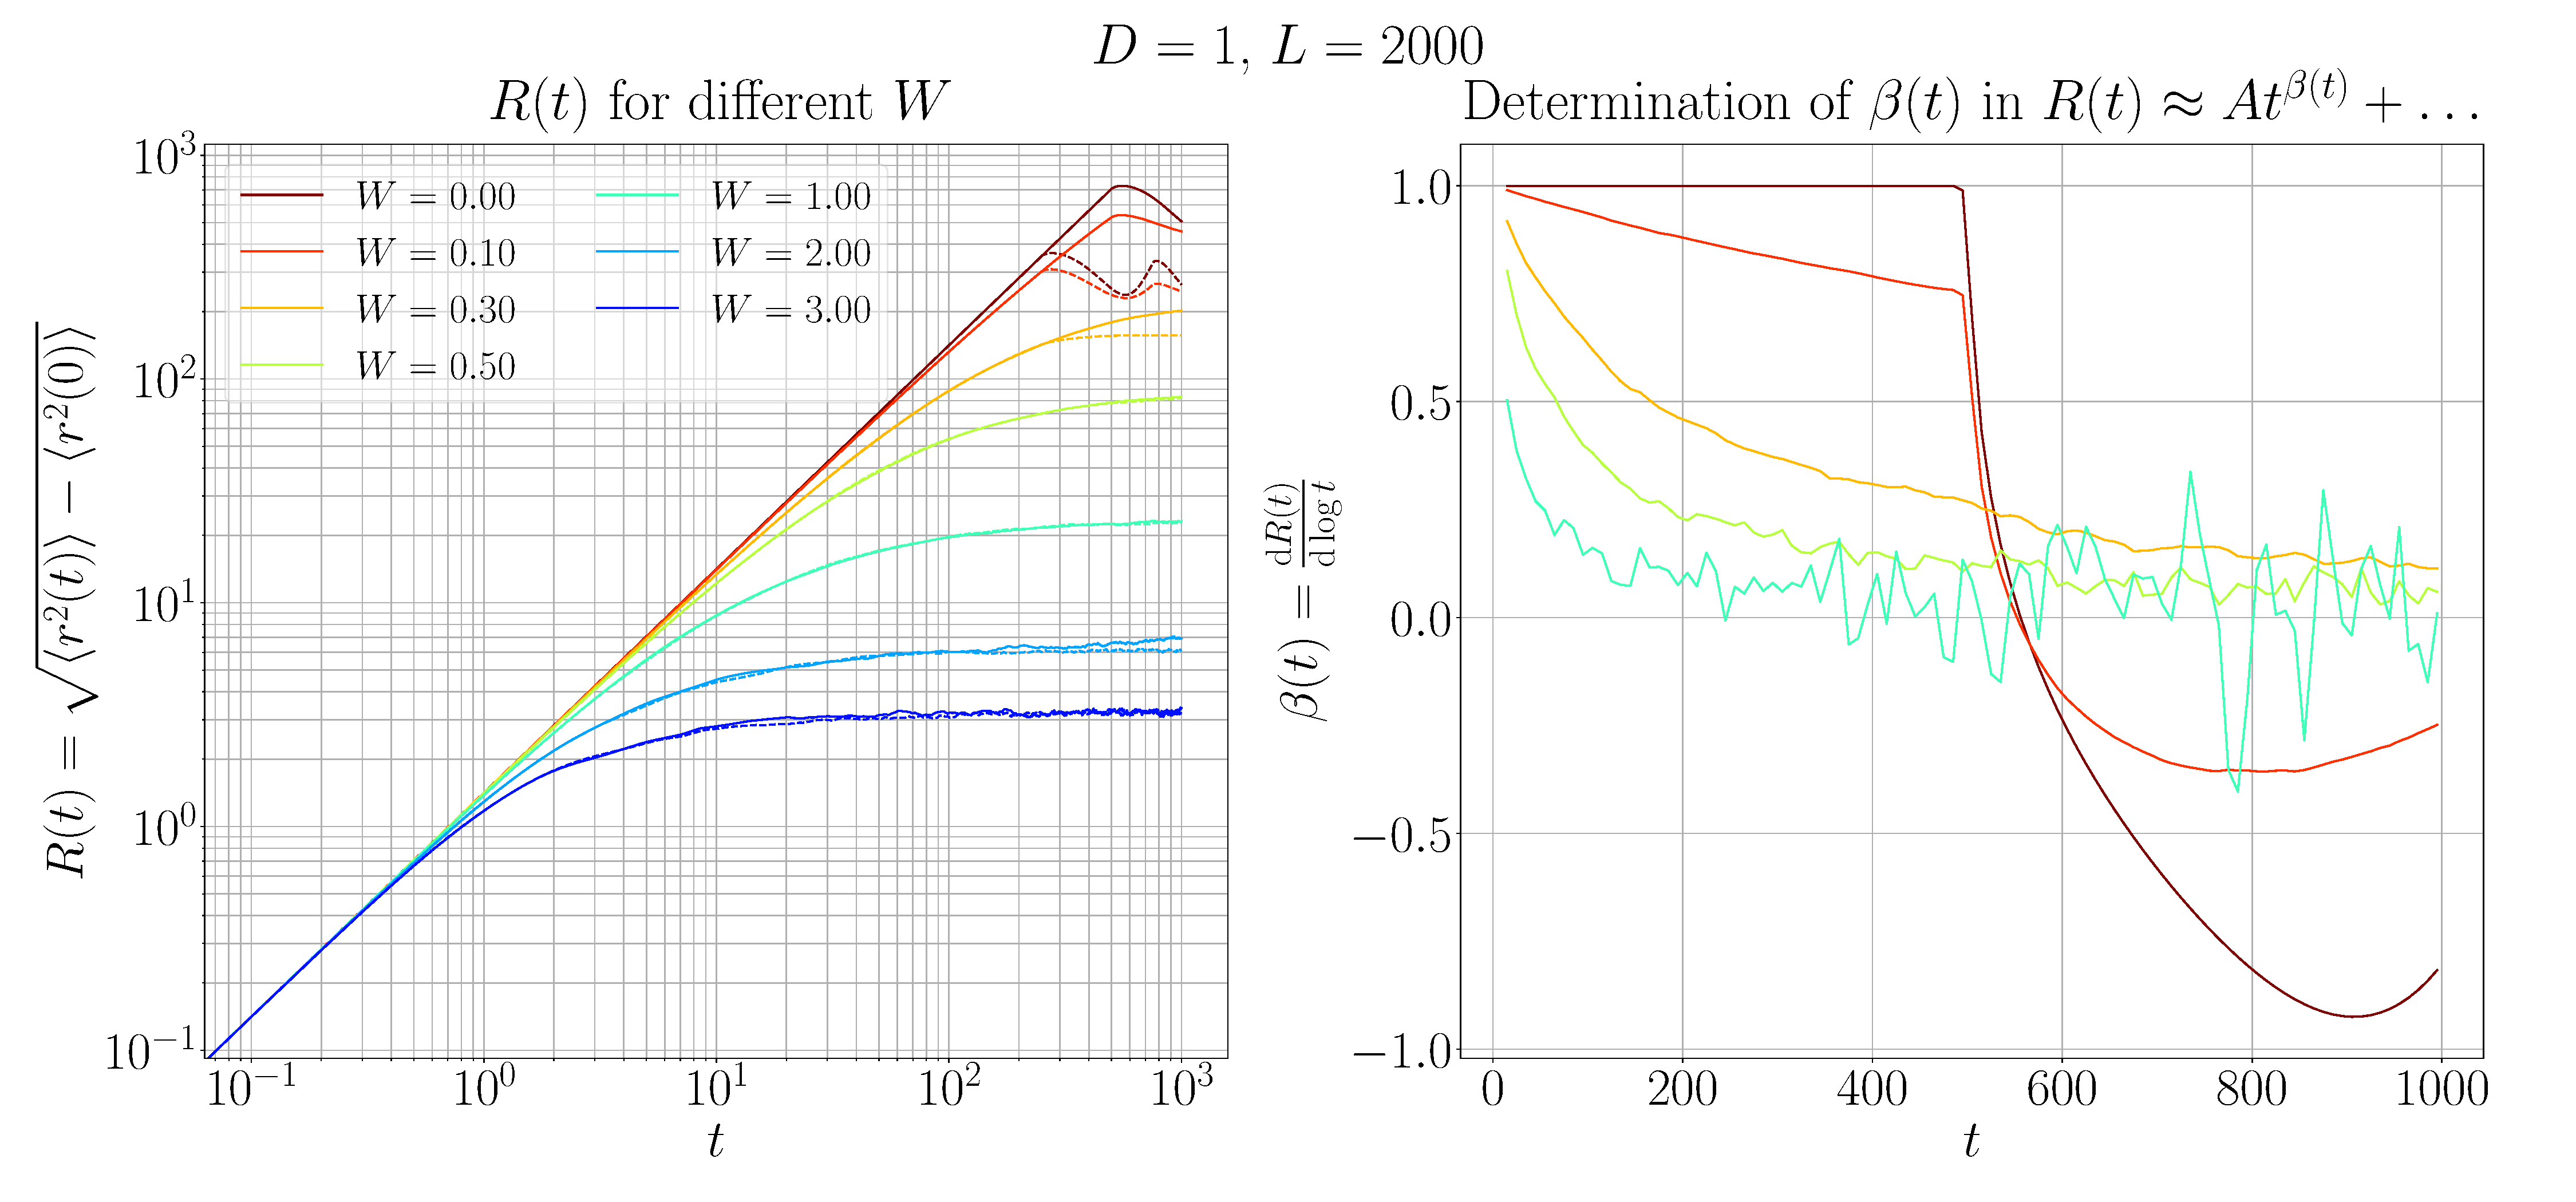
\includegraphics[width=0.8\textwidth]{1D_Anderson_localization_Seminar_scaling_analysis_D1_shape_2000_r_sq_dynamics.pdf}}
\caption{One-dimensional lattice with $L=2000$ sites. Left: time dependence of $R(t)$ averaged over 200 realizations of disorder for different values of $W$. Finite size effects are prominent in the $W=0.0$ and $W=0.1$ case, leading to a decrease in $R$ at around $t=500$ when the wave packets reached the lattice boundaries. The results for the three highest values of disorder clearly show a saturation value was reached. Dashed lines show the results of simulations on a lattice with $L=1000$ sites. Right: numerical approximation of $\beta(t)=\frac{\dd \log R(t)}{\dd \log t}$. A decreasing trend towards the value of zero is evident for finite disorder.  While curves for values of $W<1.0$ seem rather smooth, the $W=1.0$ curve shows strong fluctations, implying averaging should be performed over a greater number of samples for large $W$. Again, the $W=0.0$ and $W=0.1$ curves are only physically relevant up to $t=500$ due to finite-size effects. }
\label{fig:1D_rsq} 
\end{figure}
 
\begin{figure}[H]
\centering{
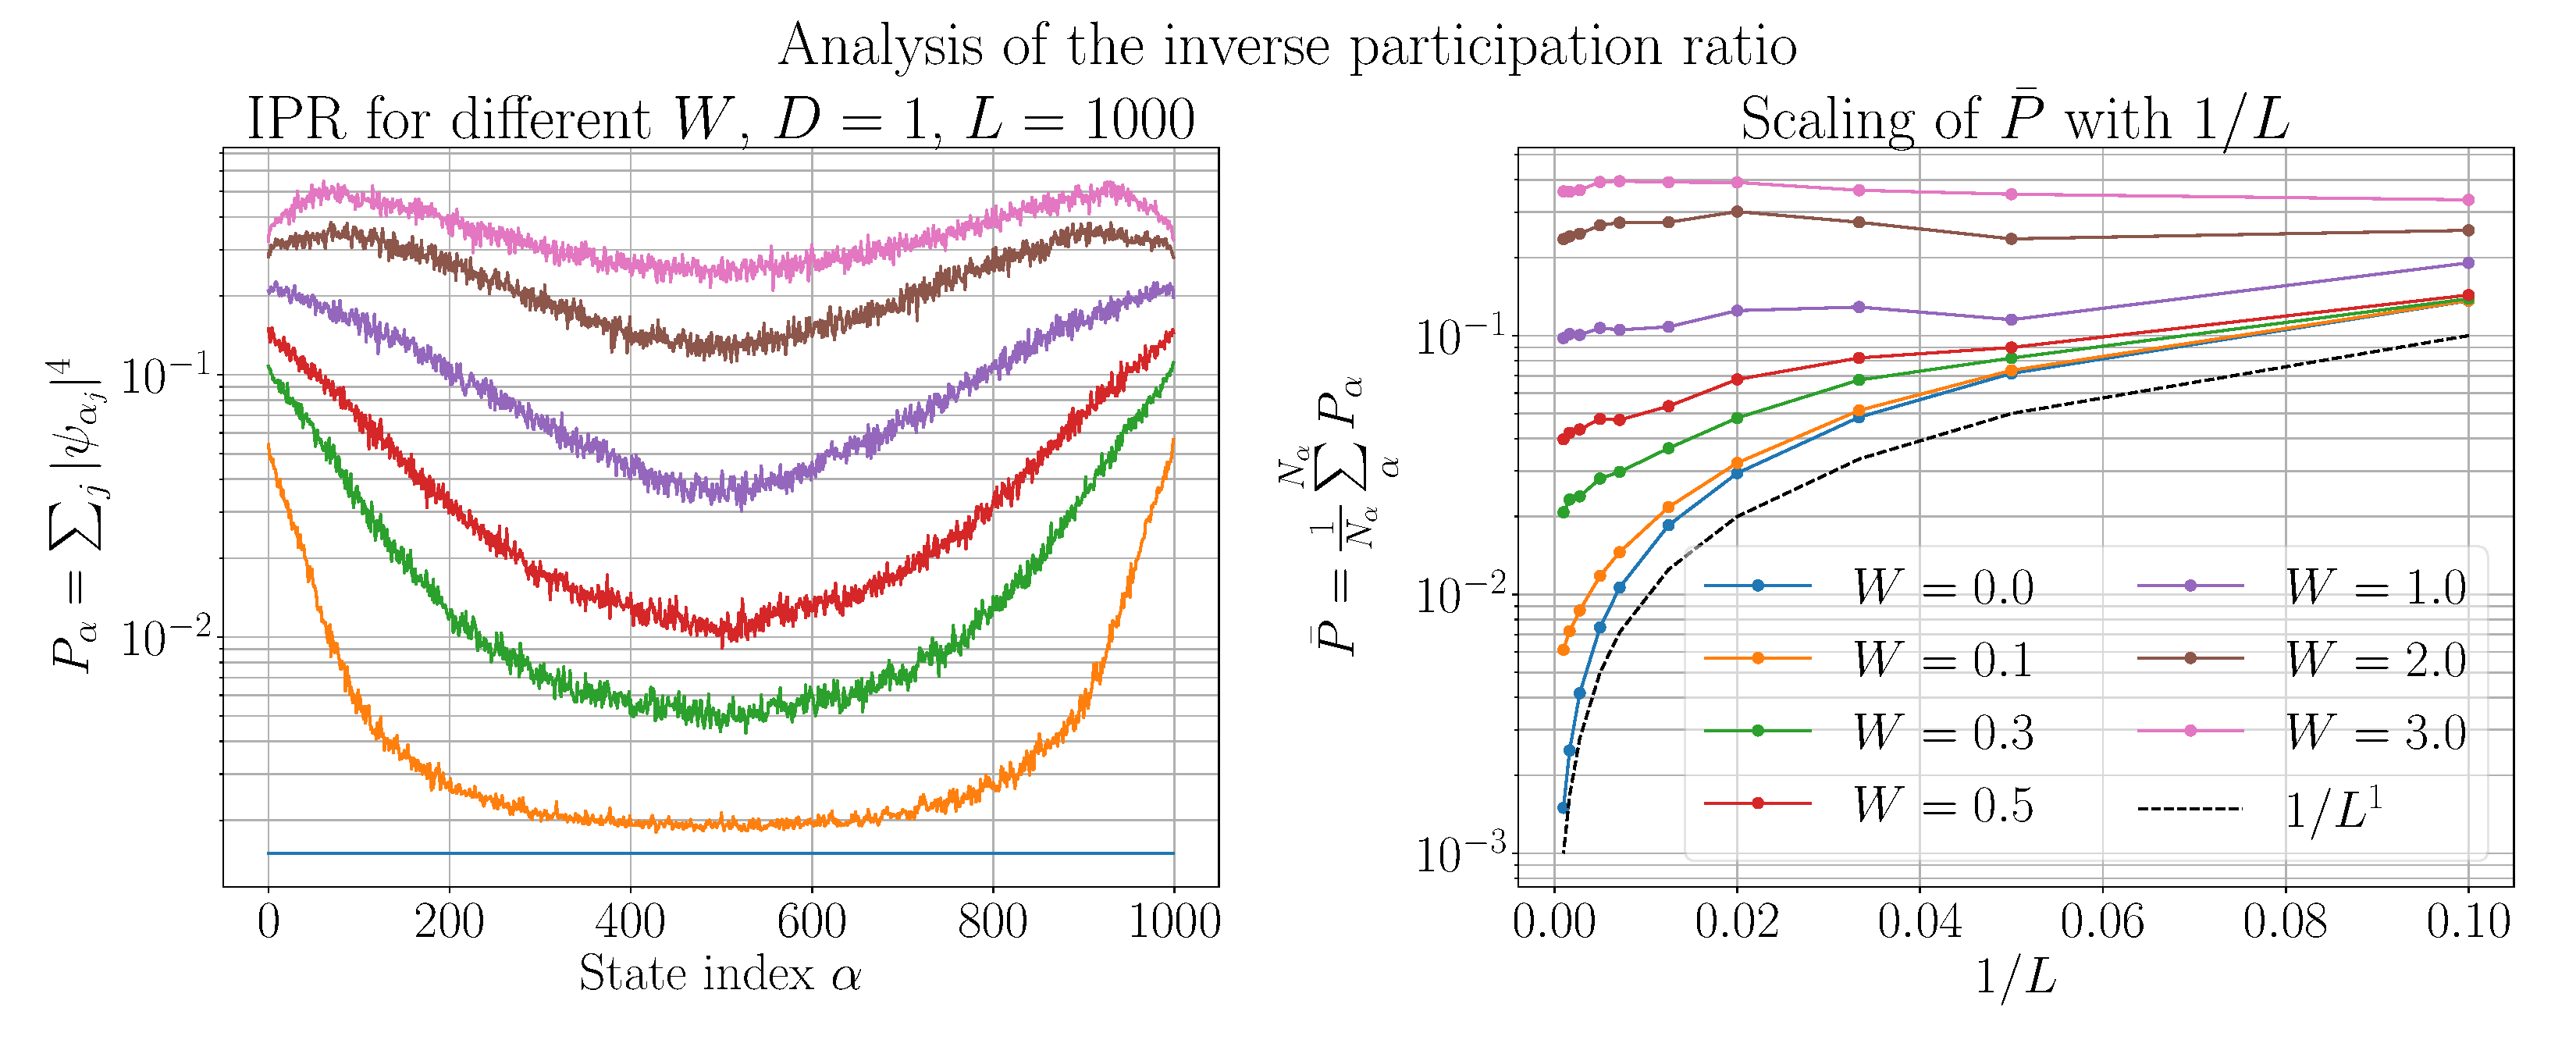
\includegraphics[width=.8\textwidth]{1D_Anderson_localization_Seminar_scaling_analysis_D1_shape_1000_ipr_plots.pdf}}
\caption{Studies of the inverse participation ratio in the one-dimensional case. Left: values of $P^{-1}_\alpha$ with respect to the eigenstate index $\alpha$ for different realizations of disorder, calculated for a lattice with $L=1000$ sites. Greater $P^{-1}_\alpha$ values mean greater degree of localization where the $W=0.0$ curve corresponds to the extended case. In accordance with the theory of the mobility edge, greater degree of localization is observed near both band edges and the curves appear symmetric with respect to the band center. In the $W=0.1$ case, the low $P^{-1}_\alpha$ values near the band center imply the states appear extended for a given system size, which is a finite-size effect. Right: finite-size scaling analysis of $\bar{P}$ given by Eq. \eqref{eq:P_ave} with respect to the inverse system size $1/L$. The results for small $L$ show that extended and localized regimes are hardly discernible in smaller systems while the difference becomes prominent once larger systems are considered.   }
\label{fig:1D_ipr} 
\end{figure}
\noindent
Above, the results of calculations in one dimension have been presented. Since the dimension of the finite Hilbert space equals the number of lattice sites, calculations in two and three dimension are much more demanding, particulary so if finite-size scaling analysis is attempted. 
% \begin{figure}[H]
% \floatbox[{\capbeside\thisfloatsetup{capbesideposition={left,center},capbesidewidth=2.3cm}}]{figure}[\FBwidth]
% {\caption{ }\label{fig:1D_ipr}}
% {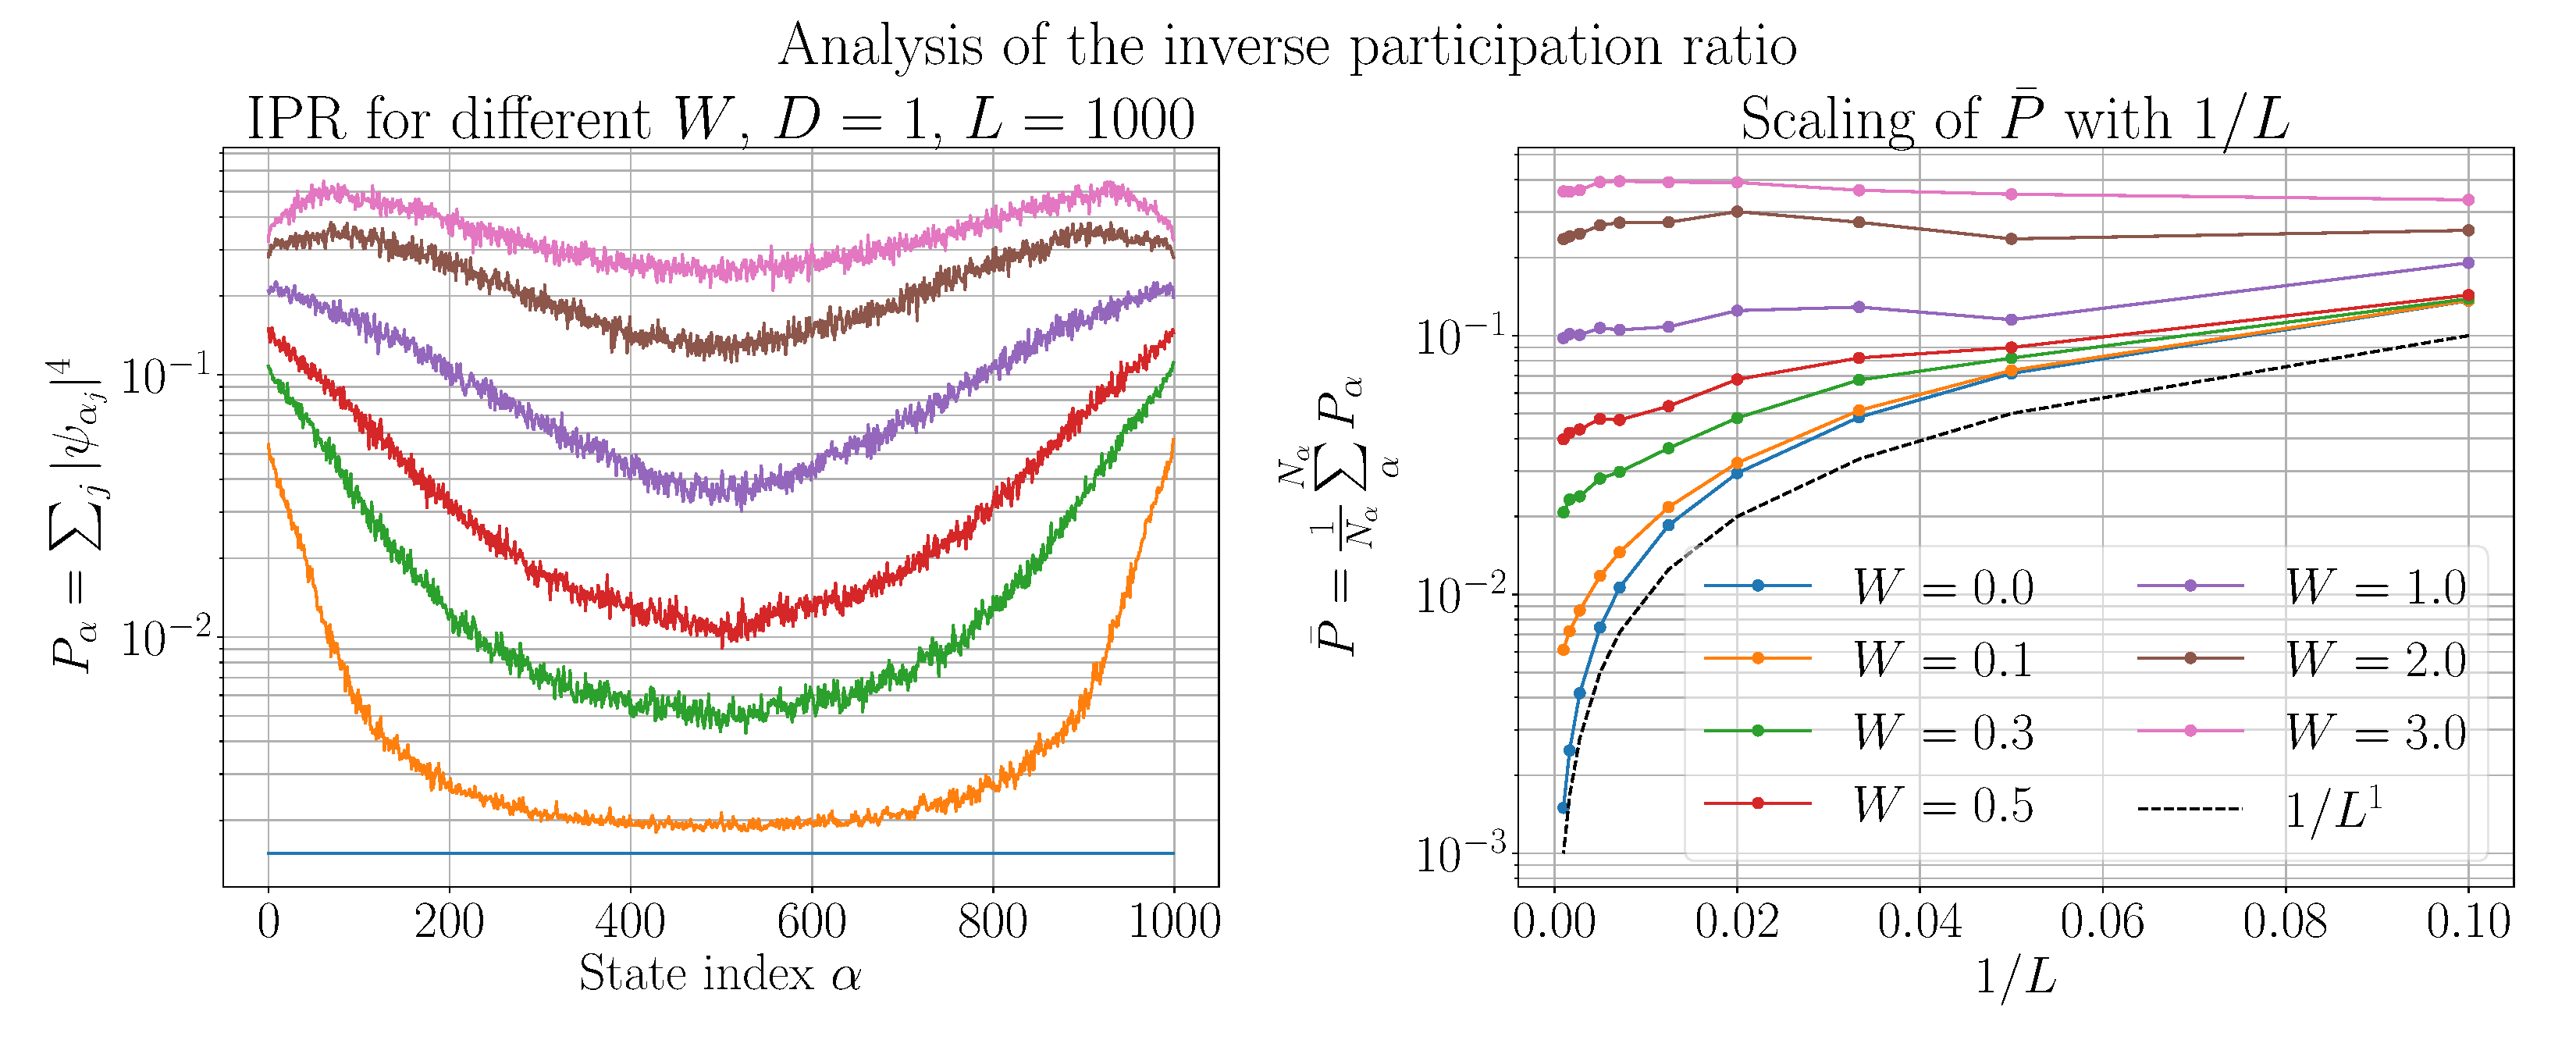
\includegraphics[width=1\textwidth]{1D_Anderson_localization_Seminar_scaling_analysis_D1_shape_1000_ipr_plots.pdf}}
% \end{figure}
\begin{figure}[H]
\floatbox[{\capbeside\thisfloatsetup{capbesideposition={left,center},capbesidewidth=3.cm}}]{figure}[\FBwidth]
{\caption{Two-dimensional lattice with $500\times500$ sites. Compared to the one-dimensional case shown in Fig. \ref{fig:1D_rsq}, it takes longer for $R(t)$ to saturate and the finite-size effects are more prominent since lattice boundaries can be reached sooner. Averaging was performed over 50 realizations of disorder.}\label{fig:2D_rsq}}
{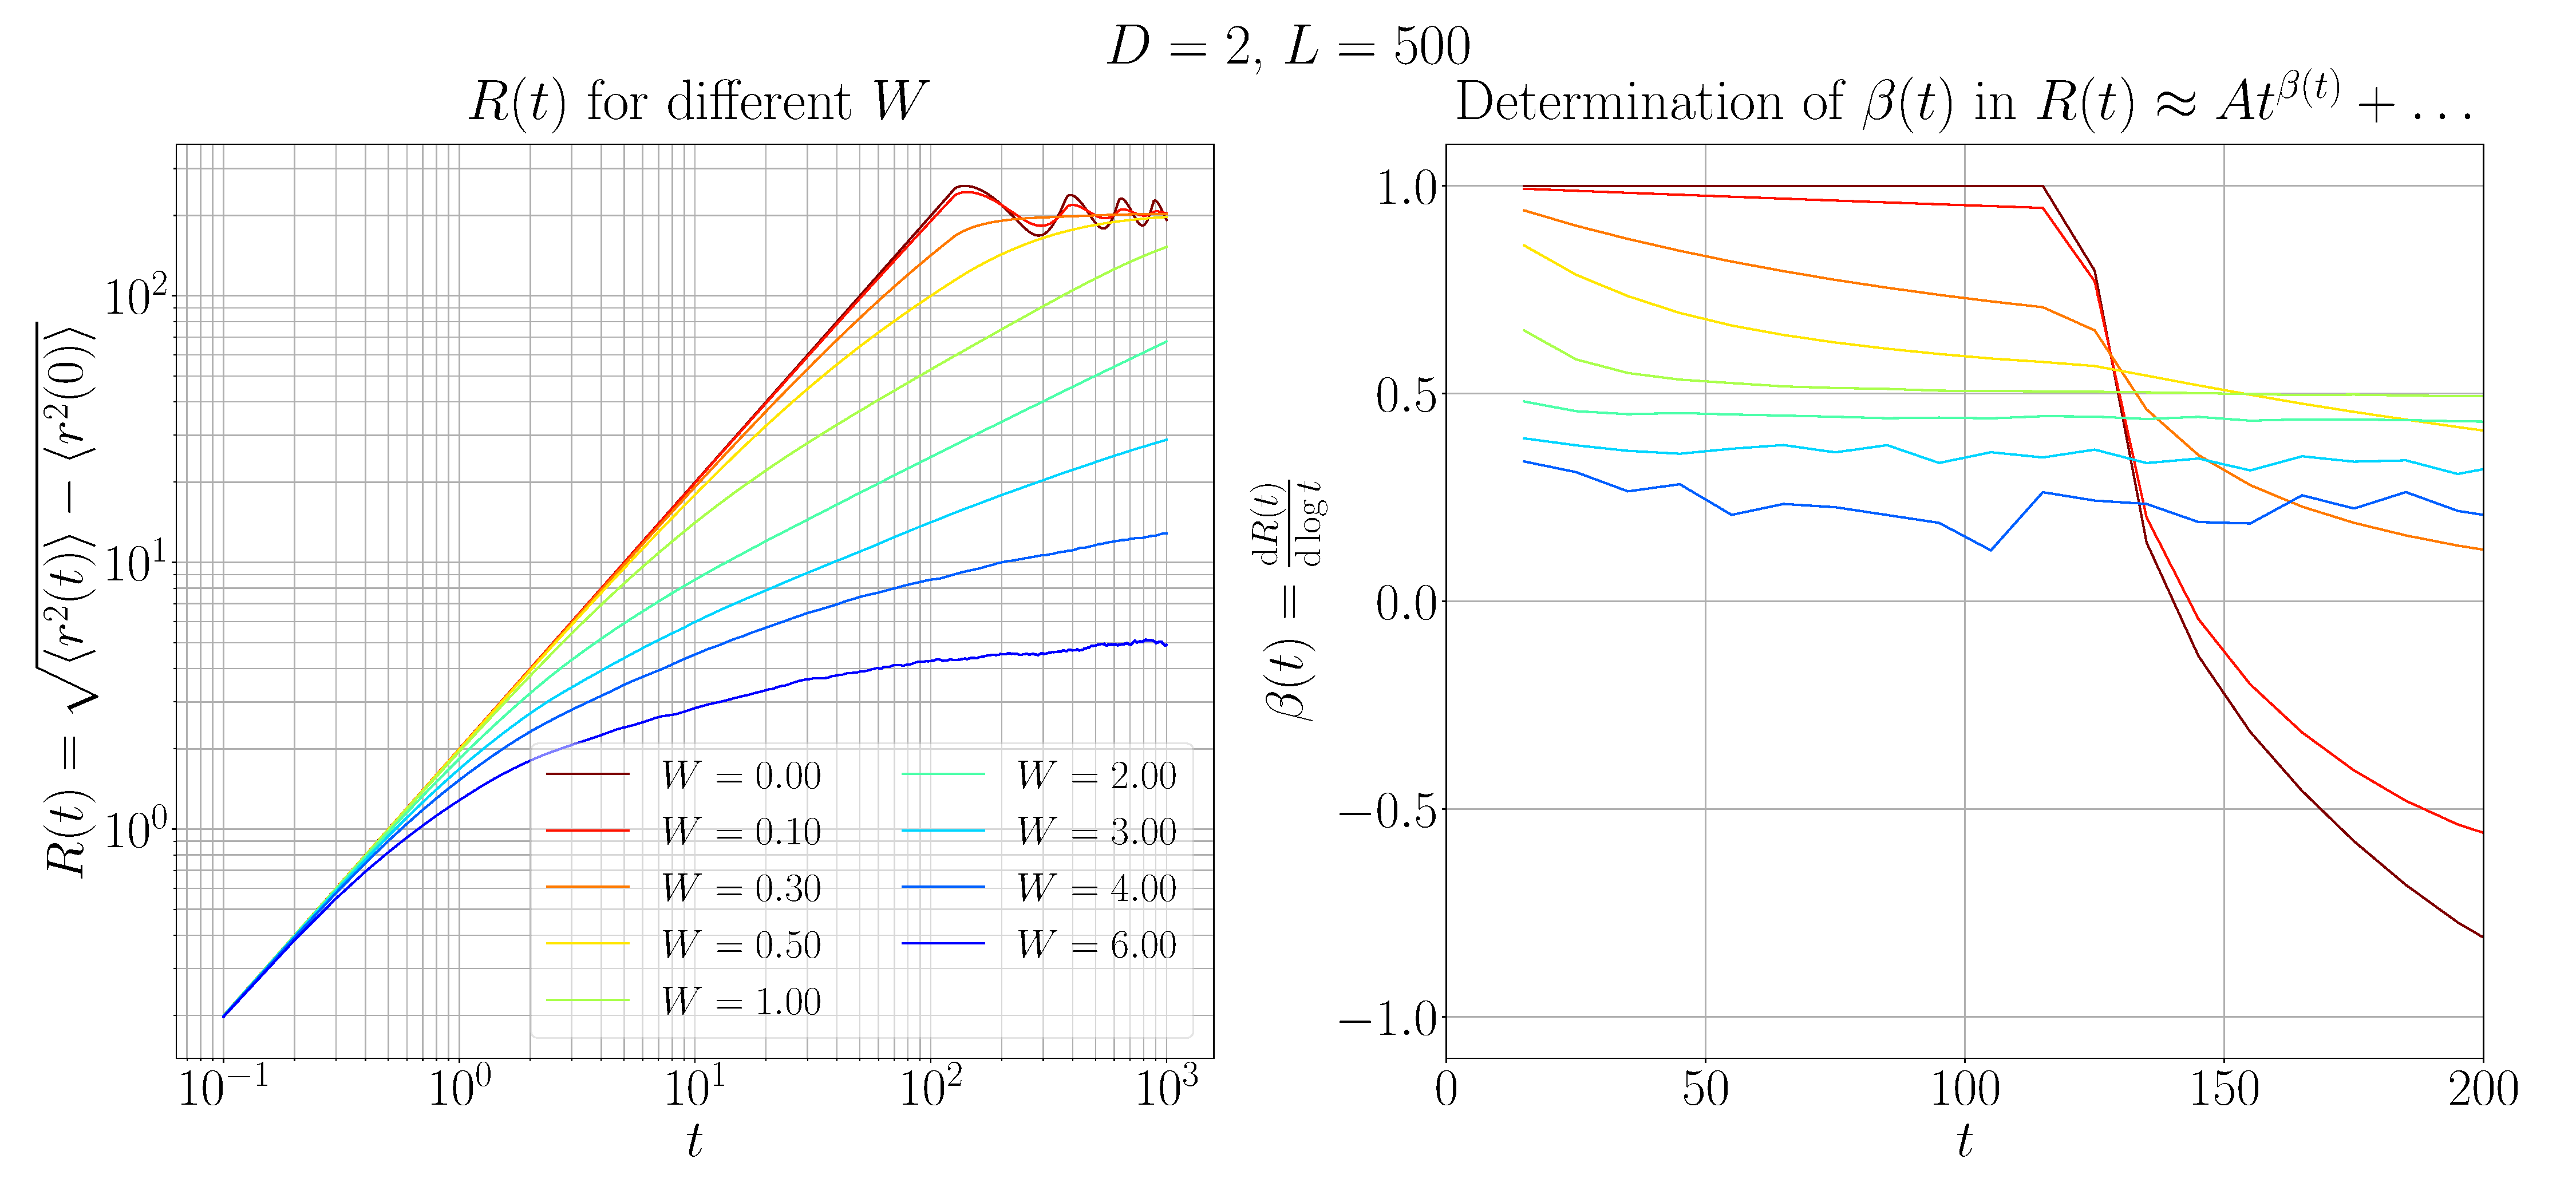
\includegraphics[width=0.8\textwidth]{2D_Anderson_localization_Seminar_scaling_analysis_D2_shape_500_500_r_sq_dynamics.pdf}}
\end{figure}
\noindent
As shown in graphs in Fig. \ref{fig:2D_rsq}, saturation of $R(t)$ occurs at a later time in two dimensions compared to the one-dimensional case. A monotonous decrease of $\beta(t)$ is observed again, while the finite-size effects appear sooner since the wave packet can reach the lattice boundaries sooner. 
\begin{figure}[H]
\centering{
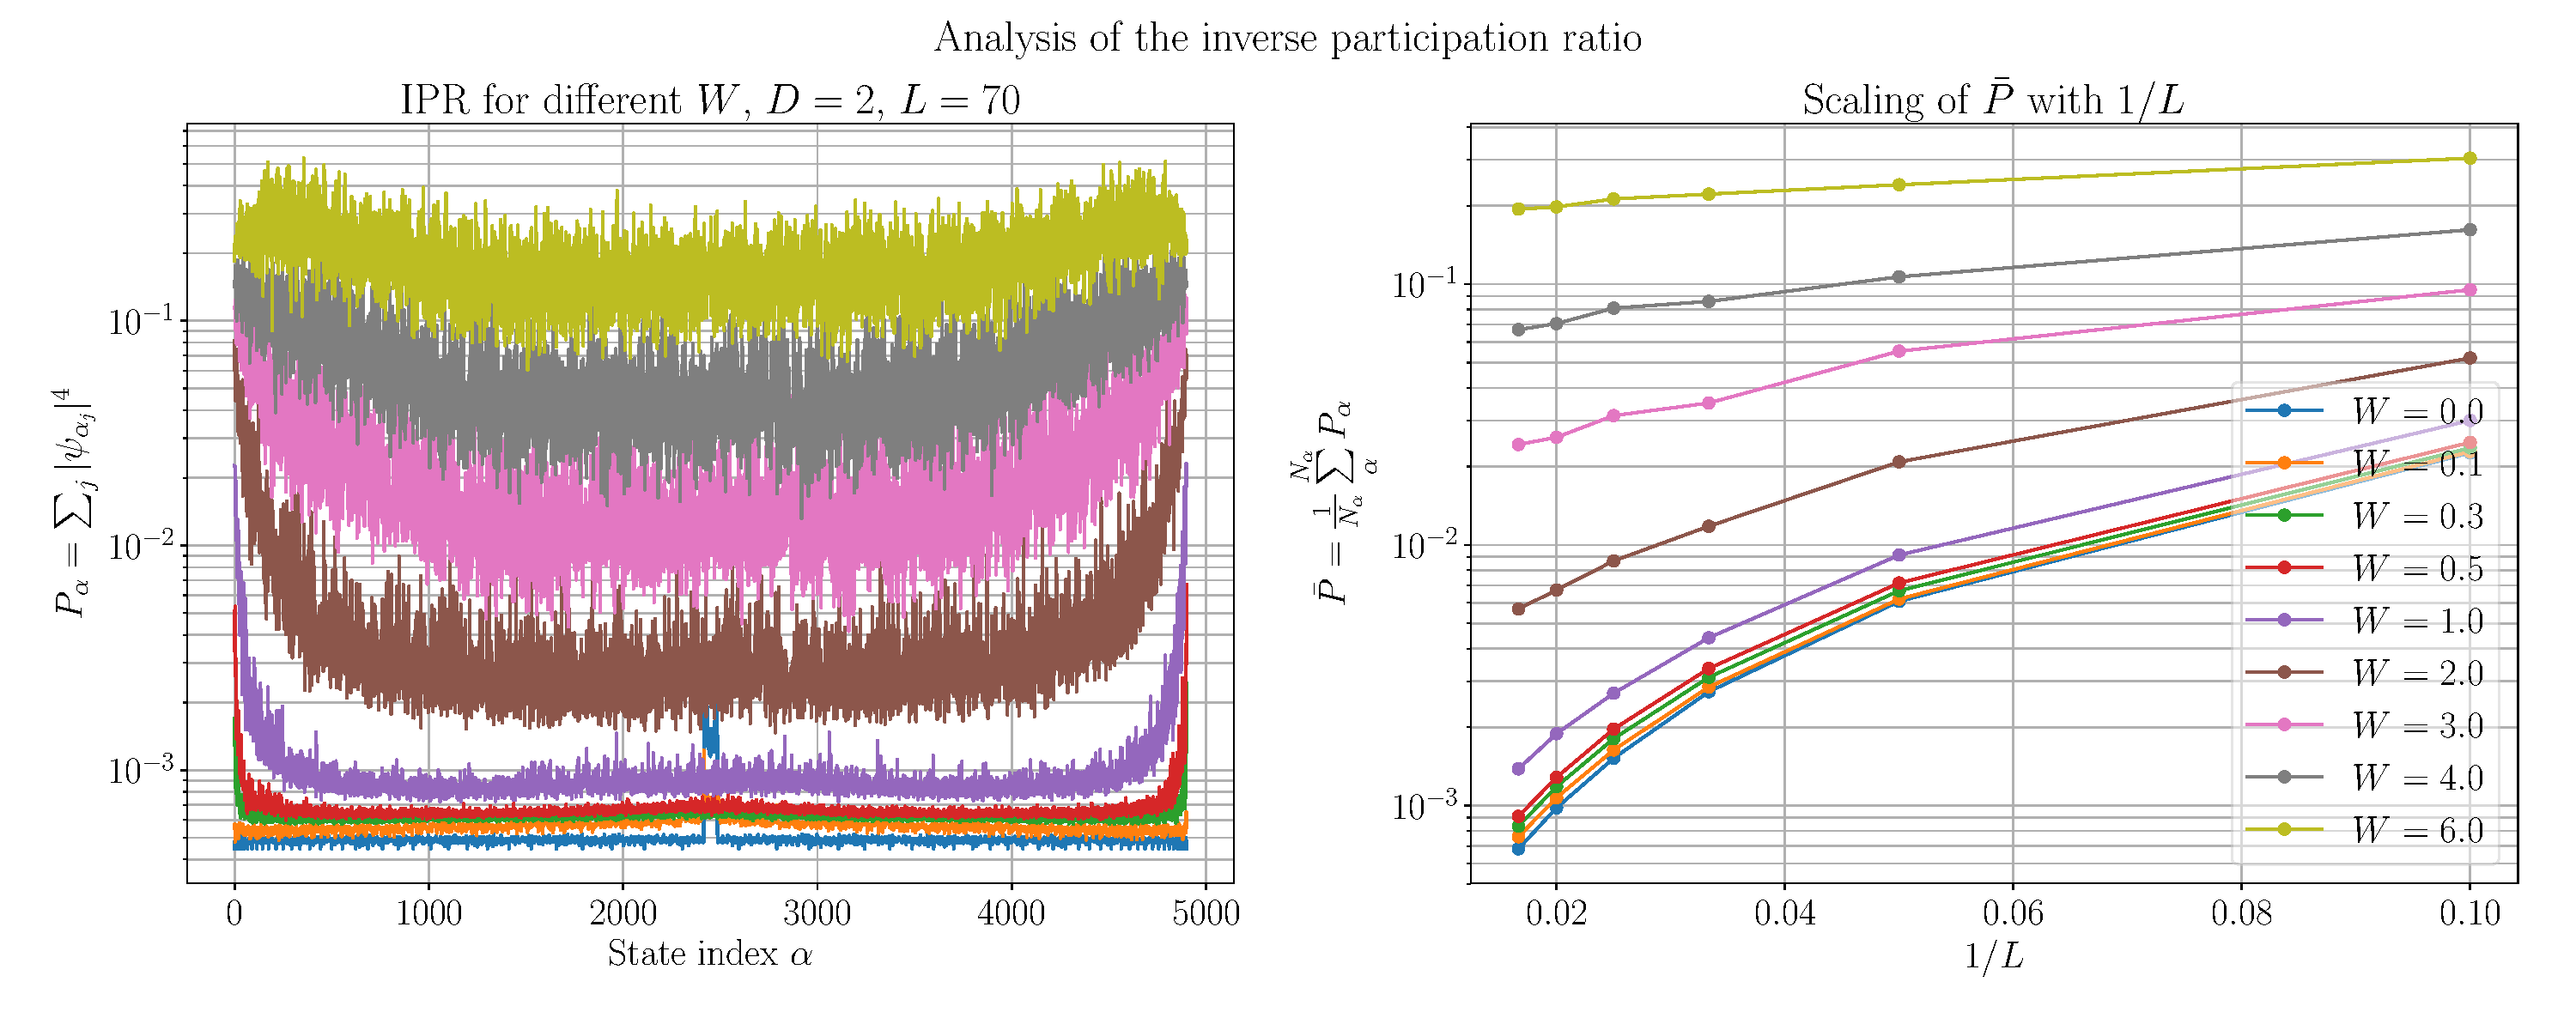
\includegraphics[width=.8\textwidth]{2D_Anderson_localization_Seminar_scaling_analysis_D2_shape_70_70_ipr_plots.pdf}}
\caption{Studies of $P^{-1}_\alpha$ and $\bar{P}$ in the two-dimensional case. Compared to the one-dimensional results shown in Fig. \ref{fig:1D_ipr}}
\label{fig:2D_ipr} 
\end{figure}
% \begin{figure}[H]
% \centering{
% 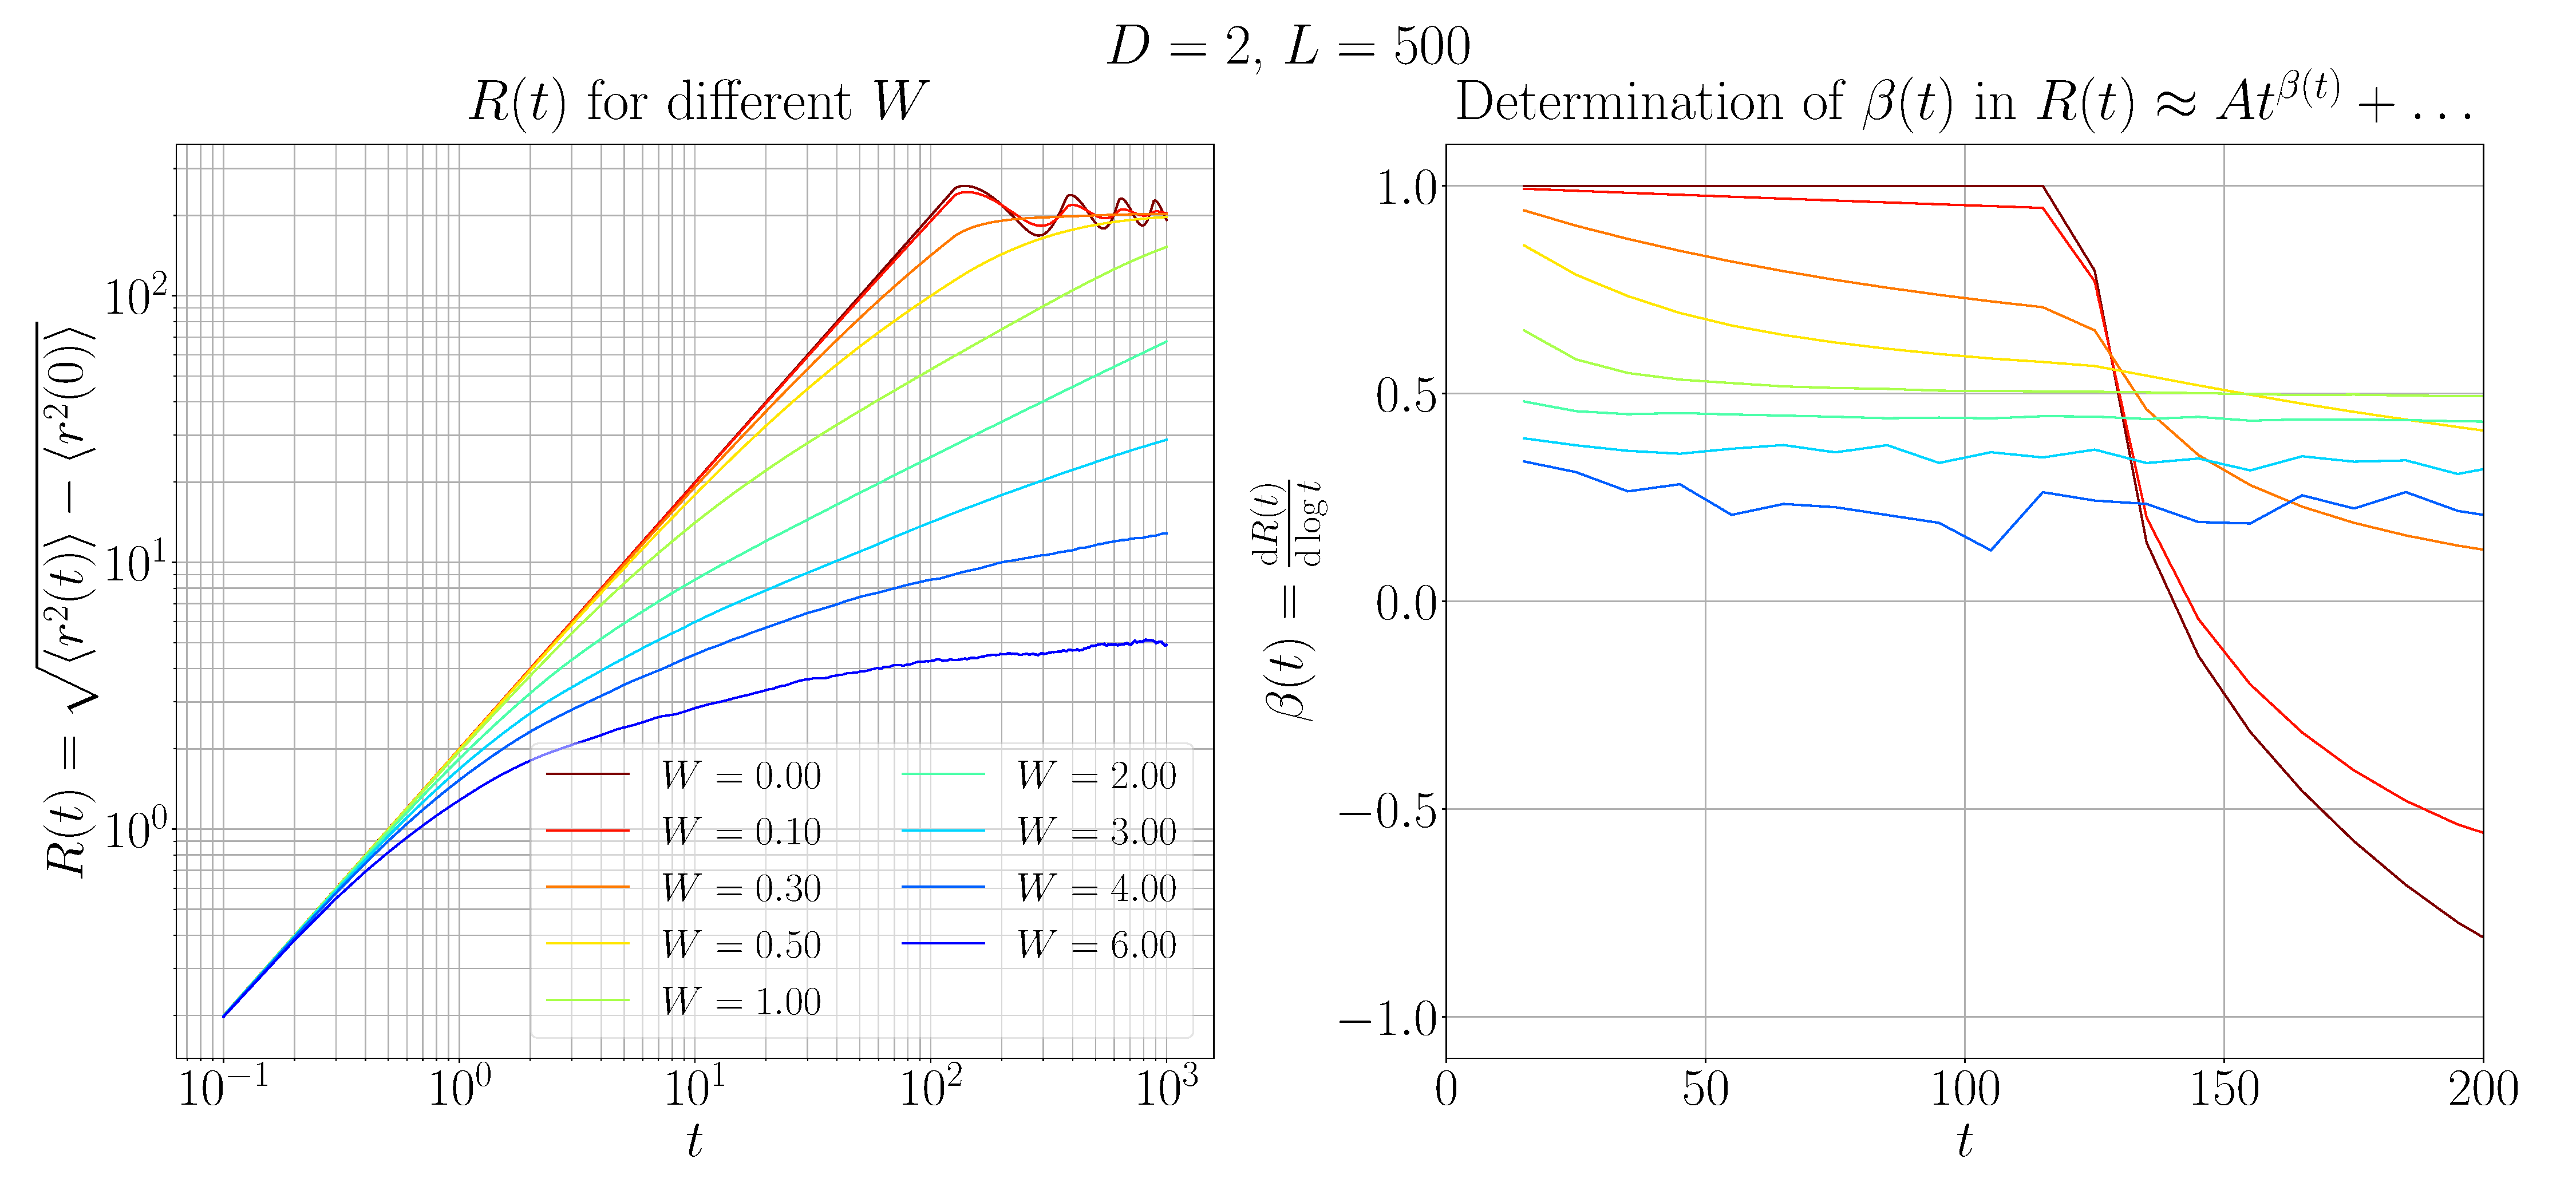
\includegraphics[width=0.8\textwidth]{2D_Anderson_localization_Seminar_scaling_analysis_D2_shape_500_500_r_sq_dynamics.pdf}}
% \caption{}
% \label{fig:2D_rsq} 
% \end{figure}
\clearpage
\begin{thebibliography}{99}
\bibitem{Anderson}
Anderson, P. (1958). \emph{Absence of Diffusion in Certain Random Lattices.} Physical Review, \textbf{109}(5), pp.1492-1505.
\bibitem{Kramer}
Kramer, B. and MacKinnon, A. (1993). \emph{Localization: theory and experiment.} Reports on Progress in Physics, \textbf{56}(12), pp.1469-1564.
\bibitem{50yearsof}
Lagendijk, A., Tiggelen, B. and Wiersma, D. (2009). \emph{Fifty years of Anderson localization.} Physics Today, \textbf{62}(8), pp.24-29.
\bibitem{Mott}
Mott, N. and Davis, E. (1971). \emph{Electronic processes in non-crystalline materials}. Oxford: Clarendon Press.
\bibitem{Abrahams}
Abrahams, E. (2010). \emph{50 years of Anderson localization.} Singapore: World Scientific.
\bibitem{Mott_Twose}
Mott, N.F and Twose, W.D (1961). \emph{Adv. Phys.} \textbf{10}, 107
\bibitem{scaling}
Abrahams E., Anderson P. W., Licciardello, D. and Ramakrishnan, T.V. (1979). \emph{Phys. Rev. Lett.} \textbf{42}, 673
\end{thebibliography}


\end{document}


